% !TeX root = RJwrapper.tex
\title{matRiks: An R package for the automatic generation of rule-based matrices}


\author{by Quietest Quokka and Bounciest Bilby}

\maketitle

\abstract{%
Few resources are available for the automatic generation of Raven-like matrices. Some of them are no longer working, while others are hardly customizable without strong programming skills. An R package fro the automatic generation of stimuli used for psychological assessment exists, but it is limited to one shape and to the manipulation of one rule (i.e., rotation). The \CRANpkg{matRiks} package has been developed with the aim of overcoming the above mentioned issues. This package can generate matrices considering different types of rules, starting from the most basic ones (e.g., changes in size, objects orientation) to the most complex ones, based on inferential and inductive reasoning. This unveils the possibility of generating new customizable stimuli and of systematically manipulating the difficulty of the matrices. Being developed within the R environment, the \CRANpkg{matRiks} package is completely open-source, allows for the reproducibility of the stimuli, and it can be easily used by people with basic knowledge of R language.
}

\hypertarget{introduction}{%
\section{Introduction}\label{introduction}}

Cattell (Cattell (1963)) defined fluid intelligence (\emph{g}) as the ability of solving novel reasoning problems that has little to do with concepts learned in schools or through acculturational processes. The adjective ``fluid'' explicitly refers to its ability to ``flow'' into a variety of tasks and cognitive activities (Horn, 1972).
Given this definition of fluid intelligence, it appears natural that the instruments for used for its evaluation tap on the respondent's ability to solve abstract problems that involve acculturation as little as possible, such as figural analogies, figure classifications, matrices, and number and letter series are often used (Horn, 1968).

The Raven's progressive matrices (RPM, JC ea Raven (1938)) are among the most famous tools for the assessment of \emph{g}. The RPM consists in a series of non-verbal multiple-choice stimuli where respondents are required to complete a series of drawings composed of different figures by identifying the relevant features that rule the relationships between the figures. These drawings are often referred to as matrices.
To pursue this aim, the respondents must choose the figure that complete the drawing among a list of other figures, the so-called distractors.
This task should measure the ability of the respondents to identify and take into account the features (also called ``rules'') that govern the relationship between the figures to compose the drawing.
The RPM and similar tasks (here denoted as Raven-like matrices or Raven-like tasks) are employed in different fields, from clinical evaluation of intelligence to the selection processes in organizational psychology (citation needed).
Since Raven's and Raven-like tasks involve the ability to solve new abstract problems, the stimuli composing these tasks should not be spread among the general population.
However, new stimuli can be generated according to the rules that govern the relationships between the figures composing the drawing. Indeed, different resources are available for developing Raven-like tasks, such as Sandia (cit), Corvus (cit), and the R package \CRANpkg{Imak} (cit).

The stimuli generated with Sandia have been analysed in an Item Response Theory framework to validate them as a test for measuring fluid intelligence.
The stimuli are available upon request to the authors, however no new stimuli can be generated because the code on which Sandia is based is no longer maintained.
Corvus represents another possible resource for generating Raven-like tasks. Corvus is written in Javascript but the Author provided a nice and easy-to-use graphical interface where the user can specify the figures and the rule(s) for the generation of the matrices. However, Corvus provides few degrees of freedom in terms of both the figures and the number of rules that can be manipulated through the graphical interface. If the user wants to add other figures, to modify the already existing figures, or to implement new rules, they have to modify the source code in Javascript, which might be a quite demanding task for people with little to null experience in programming.
Finally, the \texttt{ImaK} package is an \texttt{R} package that allows for generating visual analogies. The code for generating such stimuli (along with their response options) is quite straightforward and easy to use. However, the stimuli that can be generated with the \texttt{ImaK} package are mostly based on the rotation of the same figure to which some objects can be added or removed. As such, the only rule that is manipulated is the spatial rotation of the figures.

Given the limitations of the existing resources for generating Raven-like tasks, there might be the need of an open-source, easy-to-use, and constantly maintained resource for generating such stimuli through the systematic manipulation of rules applied to different figures.
The \texttt{matRiks} package (Brancaccio, Epifania, and de Chiusole (2023)) has been developed to pursue these aims.
Beyond generating the matrix by manipulating one or multiple rules at once on one or multiple figures, the \texttt{matRiks} package generates the response list associated to the matrix as well.
The systematic manipulation of both the rules and the figures for the matrix generation should grant the possibility of grading the granularity of the difficulty of the matrices by manipulating one element at the time.
In a similar vein, the package should allow for generating matrices that can be considered equivalent in terms of rules employed for their generation but differ in terms of figures composing the drawing. In what follows, the term stimulus is used to identify the matrix with its associated response list.

The manuscript is organized as follows.
The next section presents the rules that usually employed in the RPM along with the specific types of error responses (i.e., distractors) that compose the response list associated with a matrix. Then, the \texttt{matRiks} package is presented through an example of its application for the generation of different stimuli (i.e., the matrix with its associated response list).

\hypertarget{background}{%
\section{Background}\label{background}}

\hypertarget{rule-based-matrices}{%
\subsubsection{Rule based matrices}\label{rule-based-matrices}}

Literature highlights a plethora of rules that can be manipulated for the generation of the raven-like tasks (cit cit cit).
Beyond the fact that some of these rules have different names in different sources but refer to the same manipulation (e.g., the rule defined as ``and problem'' in Harris el a. 2020 is called ``intersection'' rule in Arendasy et al.~2005), they can be summarized into different macro-categories, namely visuospatial rules (i.e., the manipulation concerns the graphical and spatial features of the figures, Figure \ref{fig:visuoRule}), and logical rules (i.e., the manipulation concerns the logical relationships between the figures composing the matrix, , Figure \ref{fig:logiRule}). The rules can be applied (i.e., manipulated) to different figures or concatenation of figures to generate a matrix.

\begin{figure}

{\centering 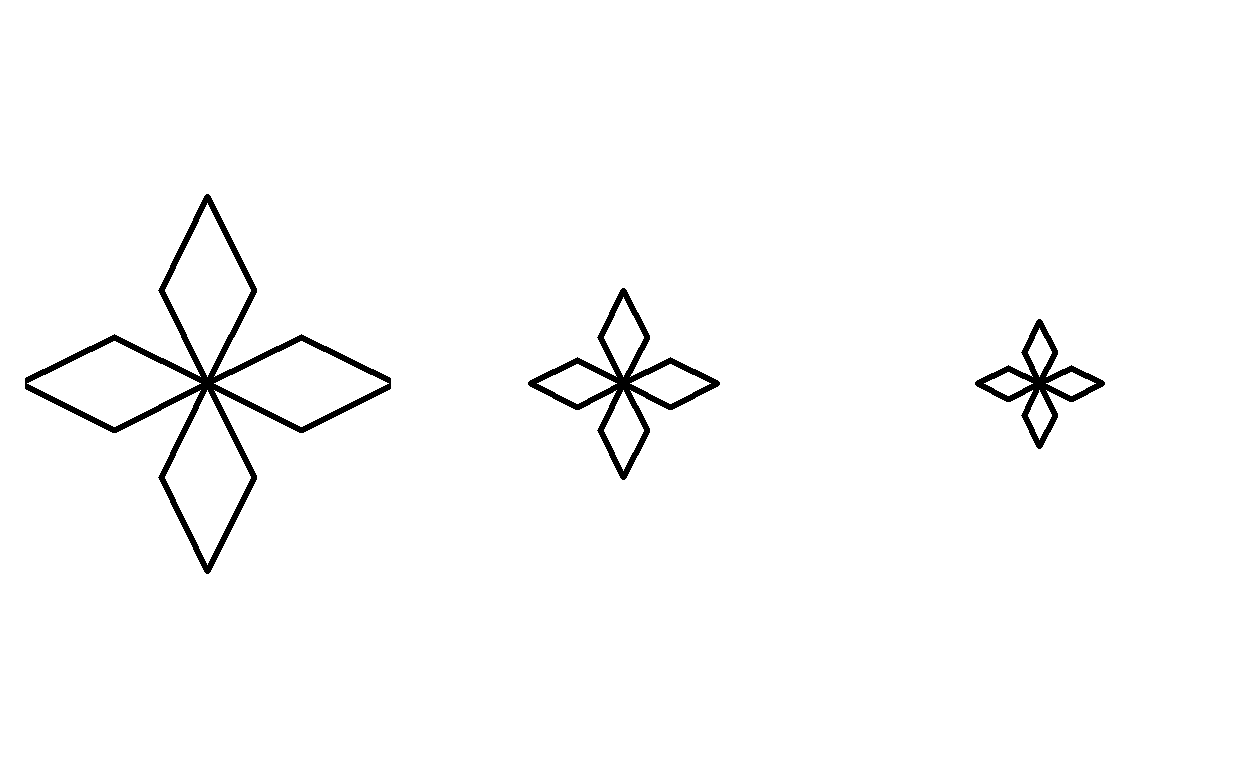
\includegraphics[width=0.7\linewidth]{matRiks-paper_files/figure-latex/visuoRule-1} 

}

\caption{Example of visuospatial rule: Changes in size}\label{fig:visuoRule}
\end{figure}

\begin{figure}

{\centering 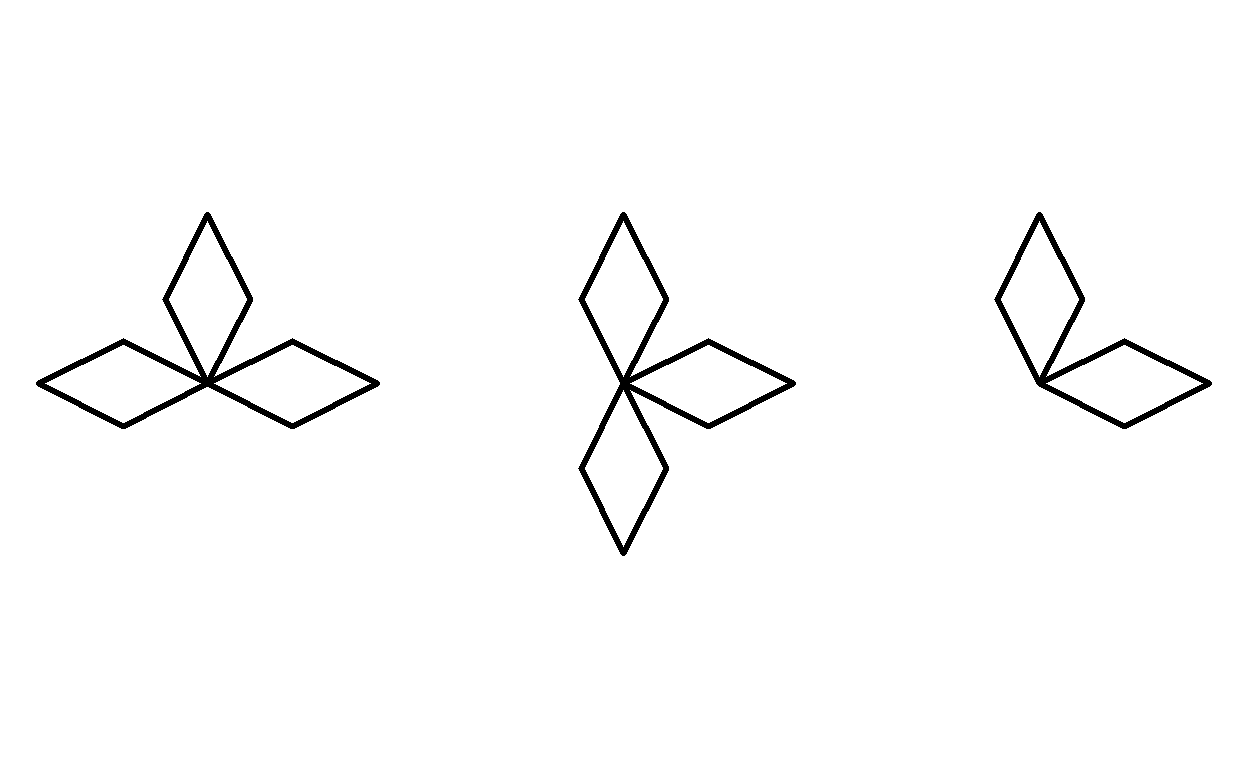
\includegraphics[width=0.7\linewidth]{matRiks-paper_files/figure-latex/logiRule-1} 

}

\caption{Example of logical rule: Insiemistic Interscetion AND}\label{fig:logiRule}
\end{figure}

In Figure \ref{fig:visuoRule}, the manipulation concerns a specif feature of the figure, that is its size, and it can be observed as the the figure decreases its size across the cells.
The rightmost cell contains the figure with the smallest size, the middle cell contains a figure with medium-small size while the leftmost object contains the figure with its original size.
In Figure \ref{fig:logiRule}, the manipulation concerns the relationships between the objects composing the figures, which are combined together according to a logical rule based on the insiemistic intersection of the objects. Specifically, the figure in the rightmost cell results from the intersection of the objects in the leftmost cell and in the middle cell.

Both visuospatial and logical rules can be manipulated according to different directional logic.
Specifically, the rules can be applied horizontally (i.e., the manipulation of the rule can be seen across columns but not across rows, H direction), vertically (i.e., the manipulation of the rule can be seen across rows but not across columns, V direction), or diagonally (i.e., the manipulation of the rule can be seen both across columns and across rows). Concerning the diagonal directional logic, it can follow either the main diagonal of the matrix (i.e., the manipulation of the rule can be seen from the top-left corner to the low-right corner, TL-LR direction) or the secondary diagonal of the matrix (i.e., the manipulation of the rule can be seen from the low-left corner to the top-right corner, LL-TR direction).

\hypertarget{the-response-options}{%
\subsubsection{The response options}\label{the-response-options}}

A large corpus of literature has investigated the role of the distractors in the response processes involved when solving the Raven matrices, focusing on the specific error response chosen by the respondent (Forthmann et al. (2020), Kunda et al. (2016), Storme et al. (2019)).
The underlying logic is that the incorrect response is not chosen at random by the respondent, but it can be the result of an educated guess, or it can be chosen because the respondent is misled for a definite reason.
In other words, the incorrect responses might reflect an incorrect solution strategy which results in the choice of a specific distractor type over another one (Kunda et al. 2016). The distractors can be classified according to the incorrect response strategy they represent.
Kunda et al. (2016) present a list of criteria for the identification of the distractors in the SPM based on the error types from the CPM and APM manuals (John Raven and Raven 2004). Specifically, the specific response that is chosen in place of the correct one (i.e.~error types) can be collected into four main four conceptual errors, namely Repetition (R), Difference (D), Wrong Principle (WP), and Incomplete Correlate (IC).
Repetition errors occur when the chosen response option is a cell adjacent to the blank space.
Difference errors occur when the chosen response option is completely different from any entry of the matrix.
Wrong principle errors occur when the chosen response option follows rules other than the ones used in the matrix. Incomplete Correlate errors occur when the chosen response option is in fact the correct response with a variation on a single feature. Each of the four main error types can be further described by their subcategories.\\
Table \ref{tab:tab-error-types-static} illustrates the definitions of the error types.

\begin{table}

\caption{\label{tab:tab-error-types-static}Taxonomy of error types}
\centering
\begin{tabular}[t]{>{}l|l|l|l}
\hline
Distractors & Definition & Specific Error & Specific definition\\
\hline
\textbf{Repetition (R)} & Entries of the matrix adjacent to the blank cell & R-Left & Repetition of the cell left to the blank space\\
\hline
\textbf{} &  & R-Top & Repetition of the cell above to the blank space\\
\hline
\textbf{} &  & R-Diag & Repetition of the cell right to the blank space\\
\hline
\textbf{Difference (D)} & Combination of all the entries of the matrix or the combination of some of their features. It is different from any entry of the matrix and from the other distractors. & D-Blank & Filled completely white or black\\
\hline
\textbf{} &  & D-Union & Some elements of one entry are emphasized\\
\hline
\textbf{} &  & D-Plus & Some entries of the matrix are combined together\\
\hline
\textbf{} &  & D-Diff & Qualitatively different from any other distractor and any entry of the matrix, resulting in a pop-out effect.\\
\hline
\textbf{Wrong Principle (WP)} & Copy or combination of the matrix entries according to another rule & WP-Copy & Repetition of a cell non adjacent to the blank space\\
\hline
\textbf{} &  & WP-Flip & Rotation or refection of one entry of the matrix.\\
\hline
\textbf{} &  & WP-Matrix & Transformation or combination of some entries of the matrix or of their elements\\
\hline
\textbf{Incomplete Correlate (IC)} & Correct response with a variation on only a single feature. & IC-Neg & Negative of the correct response\\
\hline
\textbf{} &  & IC-Fill & Correct response with a different texture or style.\\
\hline
\textbf{} &  & IC-Flip & The elements of the correct response are displayed with a different layout\\
\hline
\textbf{} &  & IC-Layout & Elements of the correct response with different proportion or different size of the correct response.\\
\hline
\textbf{} &  & IC-Scale & Correct response with a different number of elements (small layout changes are allowed)\\
\hline
\textbf{} &  & IC-Num & Correct response with a missing element.\\
\hline
\textbf{} &  & IC-Inc & Repetition of the cell left to the blank space\\
\hline
\end{tabular}
\end{table}

The criteria for the classification of the error types were used for the formal definition and generation of the distractors implemented in the \texttt{matRiks} package.
These criteria were included in the response options operator with the aim of providing the user with a response list composed of 11 elements (ten distractors and the correct response) among which they could choose the most appropriate ones.

The response options operator generates a response list composed of the correct response, three reptition distractors, one difference distractor, two wrong principle distractors, and four incomplete correlate distractors.
Further details on the formal definition of each of the distractors and on their generation are given in the ``Generation of the response list'' Section.

\hypertarget{the-matriks-package}{%
\section{The matRiks package}\label{the-matriks-package}}

The \texttt{matRiks} (Brancaccio, Epifania, and de Chiusole 2023) package can generate \(2 \times 2\) and \(3 \times 3\) Raven-like matrices with their corresponding set of responses (i.e., the correct response and all the distractors described in the Generation of response list section). The Raven-like matrices can be generated according to either visuo-spatial or logic rules, which can be concatenated with three different directional logic, namely vertically, horizontally, and diagonally.
Finally, it is possible to print the generated matrices and set of distractors as either single images (i.e., each cell of the matrix and each distractor are printed separately) or as a complete figure with the set of single distractors.

\hypertarget{installation}{%
\subsection{Installation}\label{installation}}

The \texttt{matRiks} package is available on CRAN and can be installed as:

\begin{verbatim}
install.packages("matRiks")
\end{verbatim}

The code \texttt{vignette(package\ ="matRiks")} allows for obtaining the list of all the vignettes included in the package. Each vignette can be accessed via \texttt{vignette("vignette-name",\ package="matRiks")}. For instance, the code \texttt{vignette("generate\_matriks",\ package\ ="matRiks")} opens the vignette that contains the instruction on how to generate an \texttt{RMarkdown} file where both the matrix and its associated response options are plotted together.

\hypertarget{definition-of-figures}{%
\subsection{Definition of figures}\label{definition-of-figures}}

The \texttt{matRiks} package contains a high number of default figures that can be used for the generation of the matrices.
All figures are defined as functions, hence their name has to be followed by the parentheses, and they have class \texttt{figure}.
The arguments that can be modified inside the parentheses might vary from figure to figure, and they allow for changing different features of the figure.
Specifically, the arguments that can be modified inside of the parentheses modify the default features of the figures, which are stored in a list of length 15. this list contains other lists with all the features of the figure.
The features of the figure are as follows:

\begin{itemize}
\tightlist
\item
  \texttt{shape}: character, the name of the figure
\item
  \texttt{size.x}: numeric, the length of the semi-major axis of the ellipse within which the figure is inscribed (see the documentation of the \pkg{DescTools} for further details)
\item
  \texttt{size.y}: numeric, the length of the semi-minor axis of the ellipse within which the figure is inscribed (see the documentation of the \pkg{DescTools} for further details)
\item
  \texttt{theta.1}: numeric, radiants of the rotation of the circle
\item
  \texttt{theta.2}: numeric, radiants of the rotation of the circle
\item
  \texttt{rotation}: numeric, radiants of the rotation of the ellipse within which the figure is inscribed
\item
  \texttt{pos.x}: numeric, the position on the x-axis
\item
  \texttt{pos.y}: numeric, the position on the y-axis
\item
  \texttt{lty}: integer, the line type of the margins of the figure
\item
  \texttt{lwd}: integer, the width of the margins of the figure
\item
  \texttt{num}: don't remembed
\item
  \texttt{nv}: integer, the numberof vertixes of the figures (might vary from 2 --lines-- to 100 --circle and ellipse--)
\item
  \texttt{shade}: character, the filling of a figure (can also be NA --empty figure--)
\item
  \texttt{visible}: inetger, the visibility of the figure
\item
  \texttt{tag}: character, properties of the figure used for the definition of the distractors
\end{itemize}

For instance, a simple square (Figure @ref\{fig:square\}) can be printed with the command line:

\begin{verbatim}
draw(square())
\end{verbatim}

\begin{figure}
\centering

\includegraphics{matRiks-paper_files/figure-latex/square-1.pdf}
\caption{\label{fig:square}A simple square}
\end{figure}

The figures can be summarized in different categories, and for each of these categories there is a vignette that list all the figures included in that specific category.

The following types of figure are available in the matRiks package. For each type of figures, there is a vignette availbale that lists the entire figures for each type:

\begin{figure}

\includegraphics[width=0.5\linewidth]{matRiks-paper_files/figure-latex/unnamed-chunk-2-1} \caption{[Black figures](https://cran.r-project.org/web/packages/matRiks/vignettes/black-figures.html)}\label{fig:unnamed-chunk-2}
\end{figure}

\begin{figure}
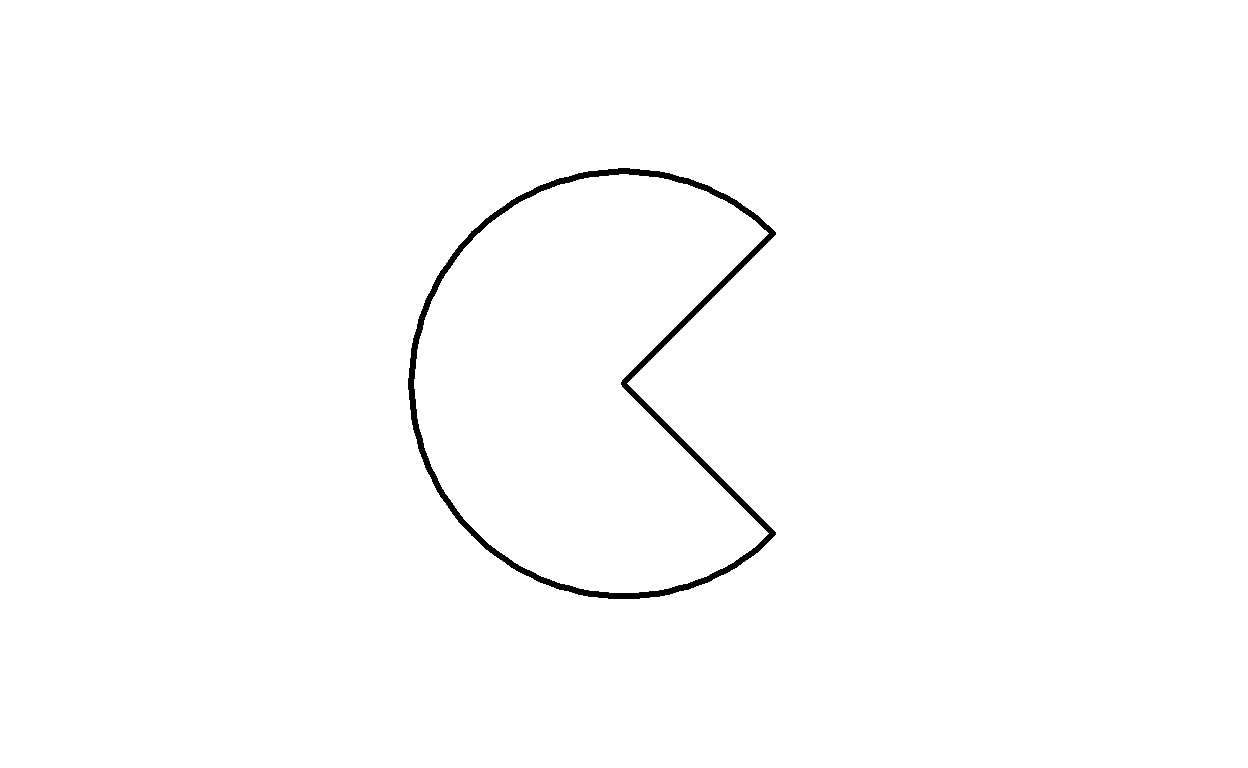
\includegraphics[width=0.5\linewidth]{matRiks-paper_files/figure-latex/unnamed-chunk-3-1} \caption{[Circle sections](https://cran.r-project.org/web/packages/matRiks/vignettes/circle-sections.html)}\label{fig:unnamed-chunk-3}
\end{figure}

\begin{figure}
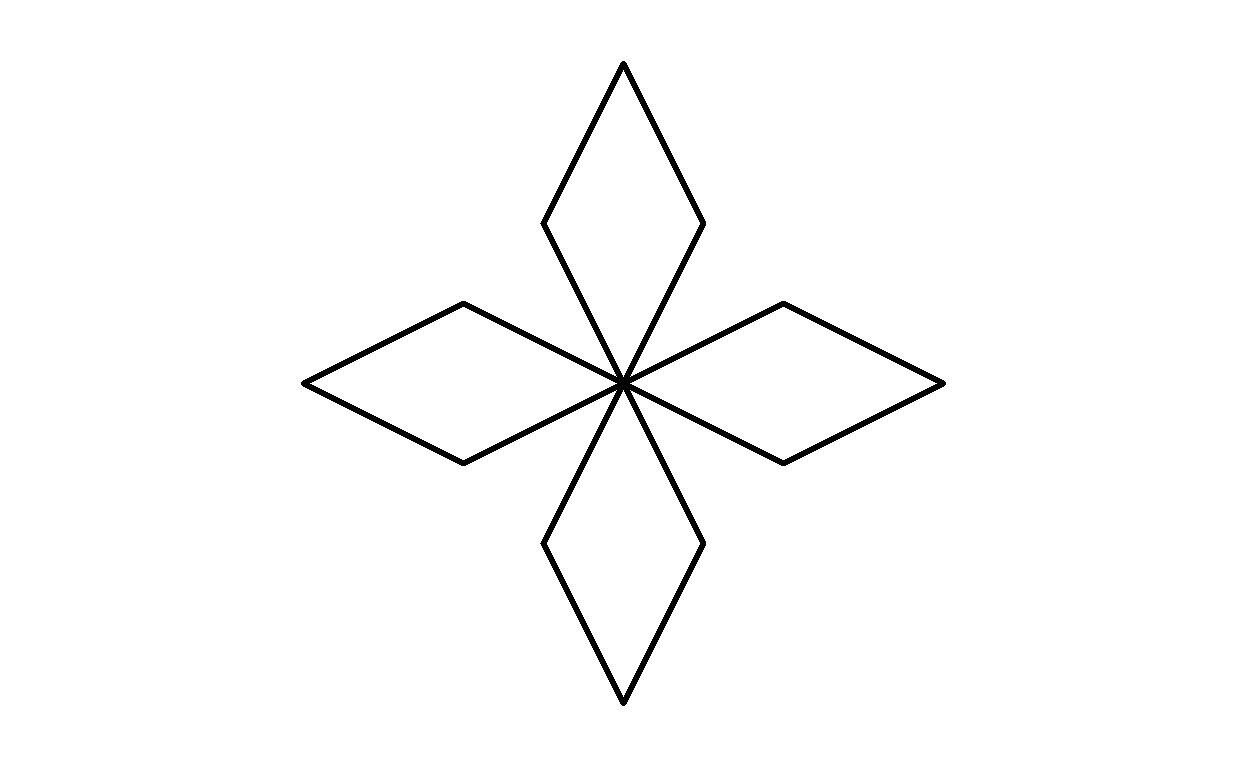
\includegraphics[width=0.5\linewidth]{matRiks-paper_files/figure-latex/unnamed-chunk-4-1} \caption{[Other figures](https://cran.r-project.org/web/packages/matRiks/vignettes/other-figures.html)}\label{fig:unnamed-chunk-4}
\end{figure}

\begin{figure}
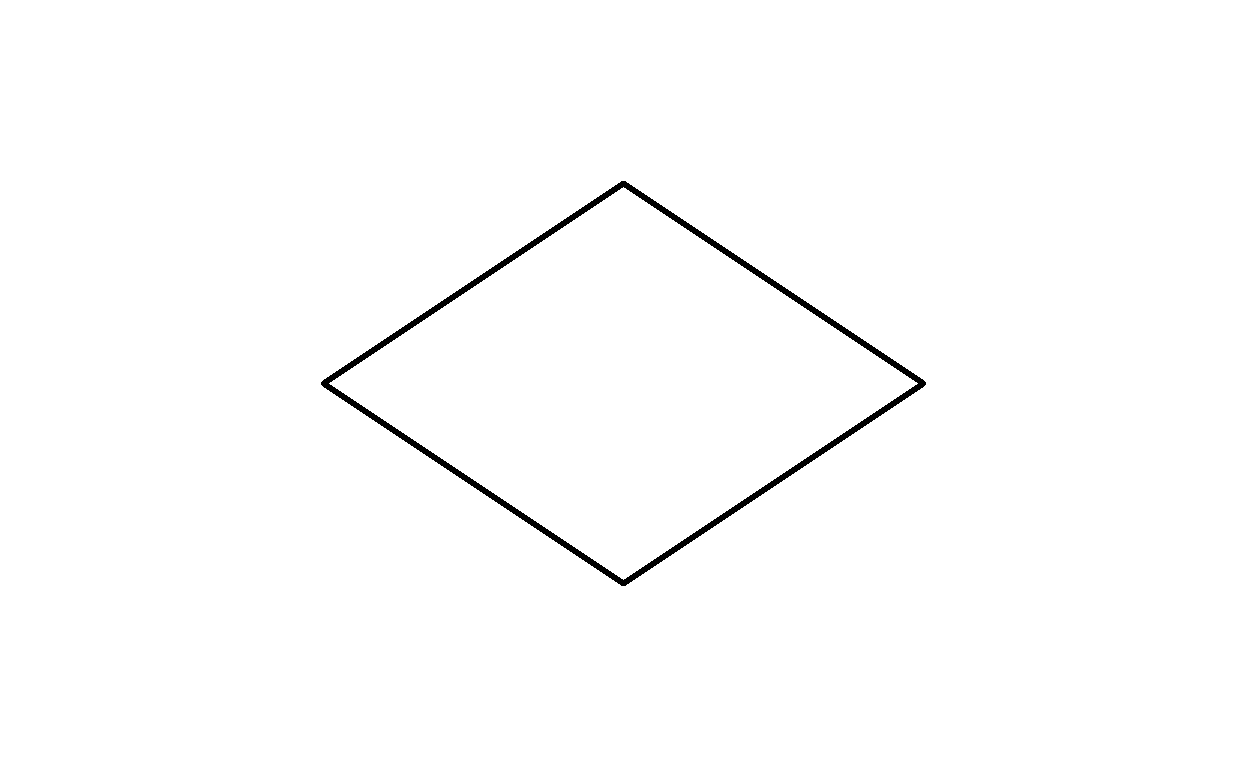
\includegraphics[width=0.5\linewidth]{matRiks-paper_files/figure-latex/unnamed-chunk-5-1} \caption{[Closed figures](https://cran.r-project.org/web/packages/matRiks/vignettes/closed-figures.html)}\label{fig:unnamed-chunk-5}
\end{figure}

\begin{figure}
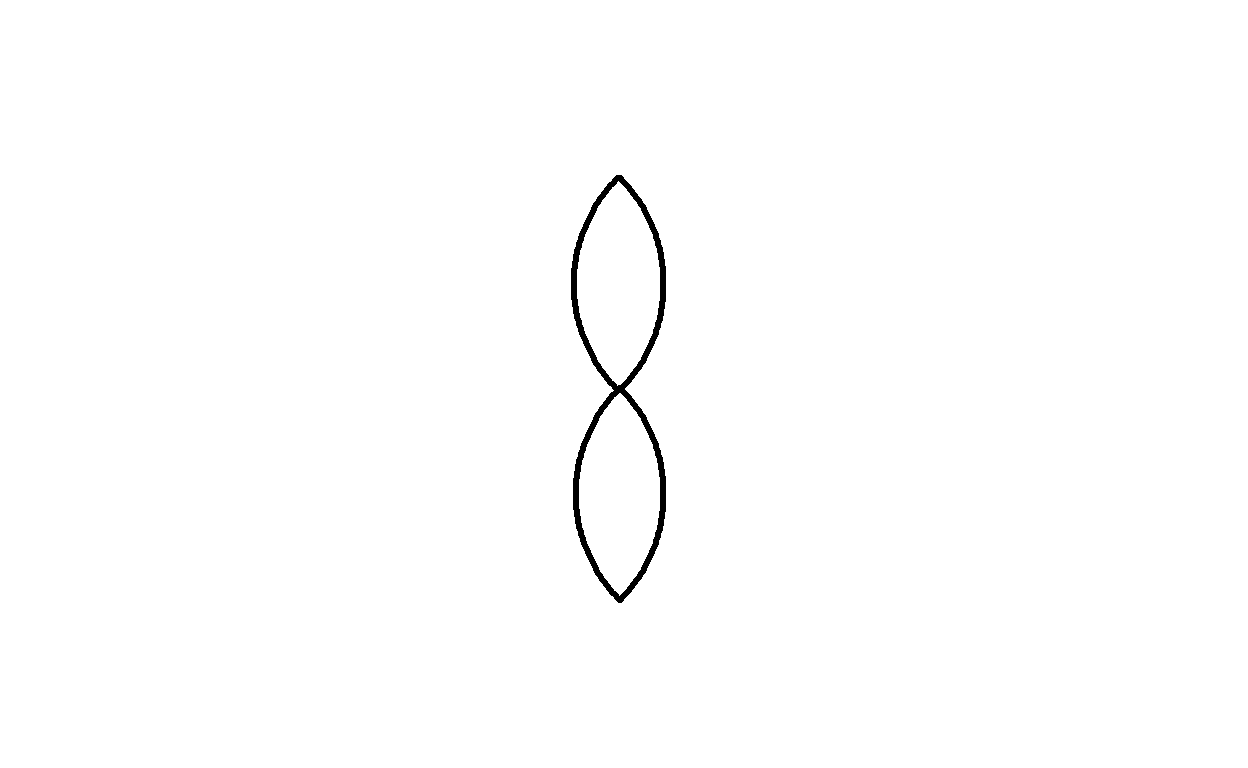
\includegraphics[width=0.5\linewidth]{matRiks-paper_files/figure-latex/unnamed-chunk-6-1} \caption{[Eight-shaped figures](https://cran.r-project.org/web/packages/matRiks/vignettes/eight-shapes-figures.html)}\label{fig:unnamed-chunk-6}
\end{figure}

\begin{figure}

\includegraphics[width=0.5\linewidth]{matRiks-paper_files/figure-latex/unnamed-chunk-7-1} \caption{[Flowers figures](https://cran.r-project.org/web/packages/matRiks/vignettes/flowers-figures.html)}\label{fig:unnamed-chunk-7}
\end{figure}

\begin{figure}
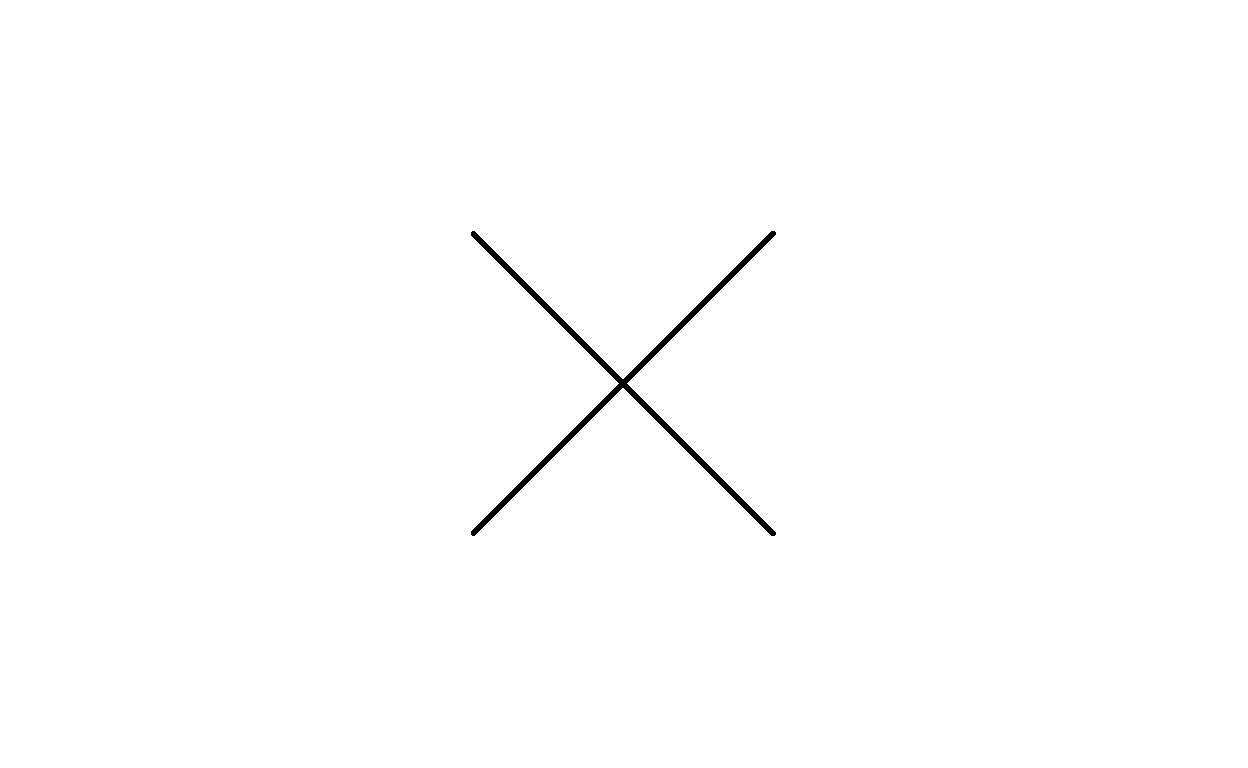
\includegraphics[width=0.5\linewidth]{matRiks-paper_files/figure-latex/unnamed-chunk-8-1} \caption{[Lines](https://cran.r-project.org/web/packages/matRiks/vignettes/lines.html)}\label{fig:unnamed-chunk-8}
\end{figure}

\hypertarget{concatenation-of-figures}{%
\subsection{Concatenation of figures}\label{concatenation-of-figures}}

Other then the pre-existing figures, the \texttt{matRiks} package allow for the generation of new figures by concatenating the existing ones. The \texttt{cof()} (\textbf{c}oncatenation \textbf{o}f \textbf{f}igures) function is designed for this aim. The arguments of the \texttt{cof()} function are the names of the default figures presented in the previous section.

For instance, the figure in Figure \ref{fig:eye} is obtained by concatenating a \texttt{circle()} and a \texttt{dot()}.

\begin{verbatim}
eye <- cof(circle(), dot()) # create the new figure eye by concatenating the circle and the dot
draw(eye)
\end{verbatim}

\begin{figure}
\centering
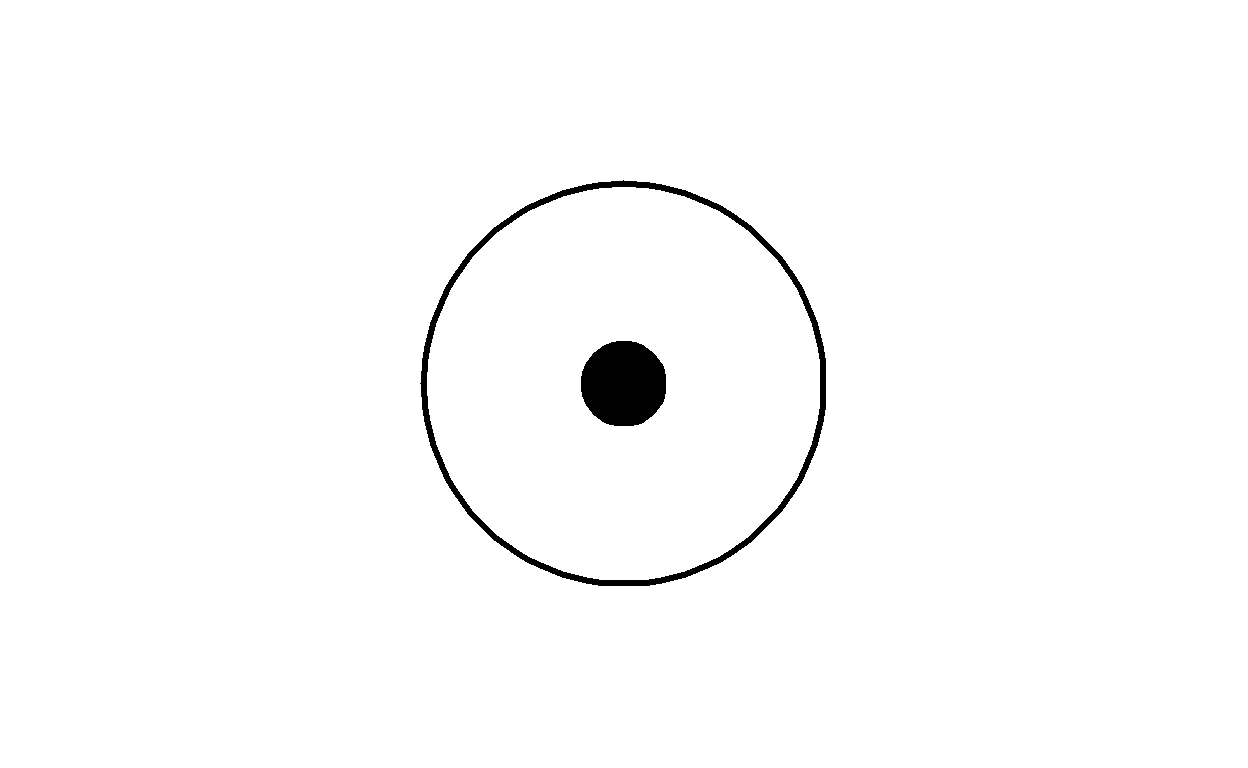
\includegraphics{matRiks-paper_files/figure-latex/eye-1.pdf}
\caption{\label{fig:eye}Example of concatenation of circle and dot to obtain an eye-like figure.}
\end{figure}

The resulting figure \texttt{eye} is a named list of lists of class \texttt{figure}. However, the two original figures are still available and can be considered as separated entities.

\begin{verbatim}
eye$shape
\end{verbatim}

\begin{verbatim}
#> [1] "circle" "dot"
\end{verbatim}

Thus, the object eye is considered a concatenation of two figures.

Function \texttt{cof()} has also two optional arguments \texttt{single} and \texttt{name}. If set to \texttt{TRUE} ,
the first argument forces the outcome of the concatenation to be consider as a new single.
The second argument defines a new name for such a figure.
The following code recreated the figure in Figure \ref{fig:eye} but it forces the new figure to be a single figle named ``eye''.

\begin{verbatim}
s_eye <- cof(circle(),dot(),single = TRUE, name = "eye")
s_eye$shape
\end{verbatim}

\begin{verbatim}
#> [1] "eye"
\end{verbatim}

This difference will be relevant for the next sections in which there are rules that require a certain number of figures to be applied.

\hypertarget{available-rules-and-matrix-generation}{%
\subsection{Available rules and matrix generation}\label{available-rules-and-matrix-generation}}

The function \texttt{mat\_apply(Sq1,\ hrules="identity",\ vrules\ ="idenity",\ mat.type=9)} is the main function for the generation of matrices based on rules and returns an object of class \texttt{matriks}.
This function allows for the generation of matrices of different dimension, either 4-cell or 9-cell matrices.
The dimension of the matrix can be specified with the argument \texttt{mat.type}, such that \texttt{mat.type\ =\ 4} results in 4-cell matrices (Table \ref{tab:fourCell-static})

\begin{table}

\caption{\label{tab:fourCell-static}Four-cell matrix}
\centering
\begin{tabular}[t]{c|c}
\hline
Sq1 & Sq3\\
\hline
Sq2 & Sq4\\
\hline
\end{tabular}
\end{table}

and \texttt{mat.type\ =\ 9} results in 9-cell matrices (default, Table Table \ref{tab:nineCell-static}).

\begin{table}

\caption{\label{tab:nineCell-static}Nine-cell matrix}
\centering
\begin{tabular}[t]{l|l|l}
\hline
Sq1 & Sq4 & Sq7\\
\hline
Sq2 & Sq5 & Sq8\\
\hline
Sq3 & Sq6 & Sq9\\
\hline
\end{tabular}
\end{table}

The \texttt{Sq1} argument defines the starting figure (i.e., the figure to be plotted in the first cell \texttt{Sq1}), which can also be a concatenation of figures. The arguments \texttt{hrules} and \texttt{vrules} allow for the definition of the directional logic with the rule(s) is applied, such that the rules specified in \texttt{hrules} are manipulated horizontally and those specified in \texttt{vrules} are applied vertically.

The application of the \texttt{mat\_apply()} function results in an object of class \texttt{matriks}, which is a named list. The length of the list vary as the dimension of the matrix varies, such that it has length 7 when \texttt{mat.type\ =4} and of length 12 otherwise. Regardless of the length of the list, it contains the characteristics of the matrix. the following example is based on a 9-cell matrix where the identity rule was applied both horizontally and vertically:

\begin{verbatim}
#>  [1] "Sq1"      "Sq2"      "Sq3"      "Sq4"      "Sq5"      "Sq6"     
#>  [7] "Sq7"      "Sq8"      "Sq9"      "hrule"    "vrule"    "mat.type"
\end{verbatim}

In particular, \texttt{Sq1} to \texttt{Sq9} are lists containing the figures for each of the nine cells composing the matrix, while \texttt{hrule}, \texttt{vrule}, \texttt{mat.type} are vectors containing the rules applied the rules applied horizontally, vertically, and the dimension of the matrix, respectively. Since this is a 9-cell matrix, the list is of length 12 and it contains the cells from Sq1 to Sq9. If a 4-cell matrix is generated, then the list if of length 7 and it contains the cells from Sq1 to Sq4, along with \texttt{hrule}, \texttt{vrule}, \texttt{mat.type} .

The rules are methods that transform a feature of the figure to obtain a different figure or a figure with a modified feature.
The \texttt{matRiks} package implements several rules, each of which may be classified differently.
The table contains all the rules available in the package, their descriptions, and classifications.

{[}Rule table {]}

As already mentioned, the rules can be classified into visuospatial and logical rules.
Such macro classification may have an impact on the difficulty of the generated matrix {[}cita{]}.
By the way in which the rules have been defined in the \pkg{matRiks} package, they can be either incremental or permutational rules.

The operation underlying the functioning of the incremental rules is the increment of a fixed quantity.
Incremental rules apply a fixed increase (or decrease) on each cell of the matrix to obtain the feautures of the figure in the following cell, starting from the first cell.
The order in which the fixed increase (decrease) is applied depends on the directional logic used for the generation of the matrix.
For instance, Figure \ref{fig:incremental} illustrates the application of the change in size rule on a square. the change in size rule is an incremental rule, in which the size of the square decreases of a fixed quantity in each subsequent object according to a directional logic.

\begin{figure}
\centering
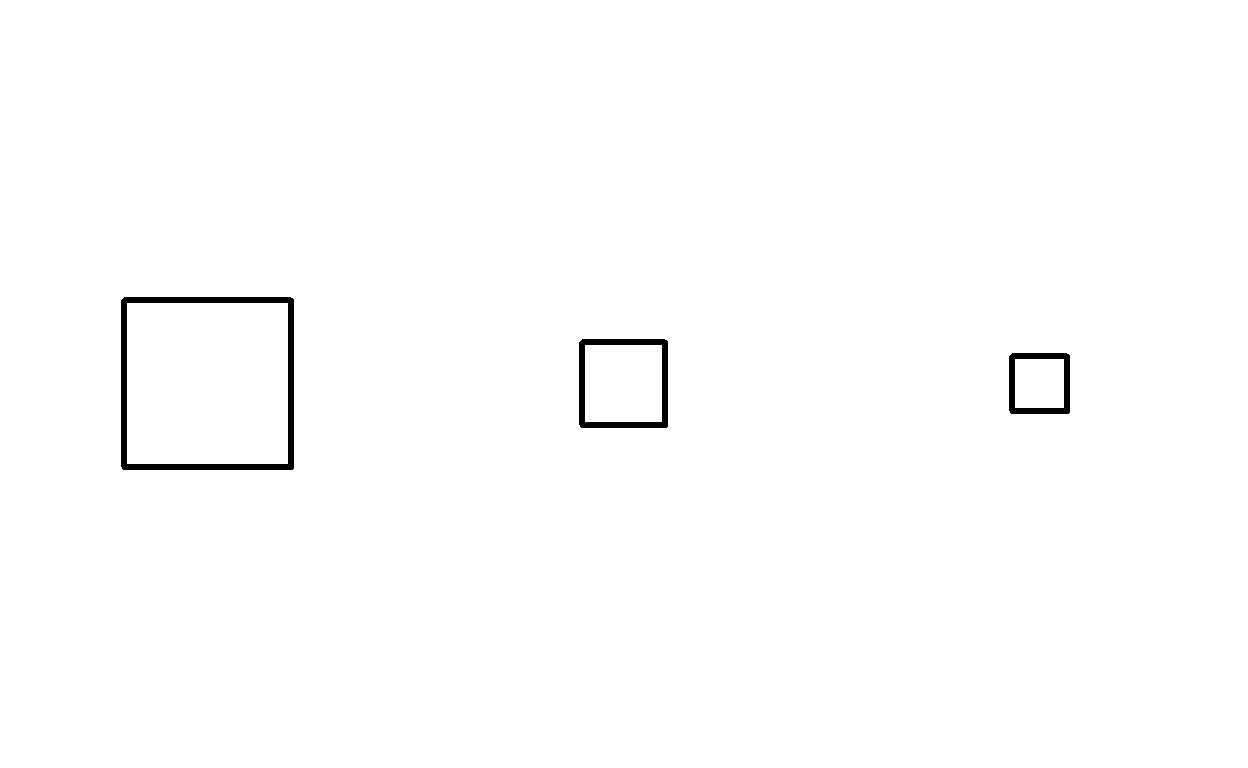
\includegraphics{matRiks-paper_files/figure-latex/incremental-1.pdf}
\caption{\label{fig:incremental}Example of size rule transformation along a row.}
\end{figure}

The incremental aspects appear because the squares are smaller compared to the ones on their right but larger than the ones on their left.
Hence, by changing the position of any figure in the row the results would not necessarily respect the definition of the rule.

The operation underlying the functioning of the permutational rules is the permutation of the figures (or of their features) across the cells according to a directional logic.
For instance, the change in shapes rule is a permutational rule where the objects shown in each cell of the matrix are permuted following an order that is consistent with the directional logic.
For instance, consider a matrix where a set of three figures (\texttt{hexagon()}, \texttt{pentagon}, \texttt{square}) are manipulated according to the shape rule following an horizontal directional logic (Figure \ref{fig:permutational}).

\begin{figure}
\centering
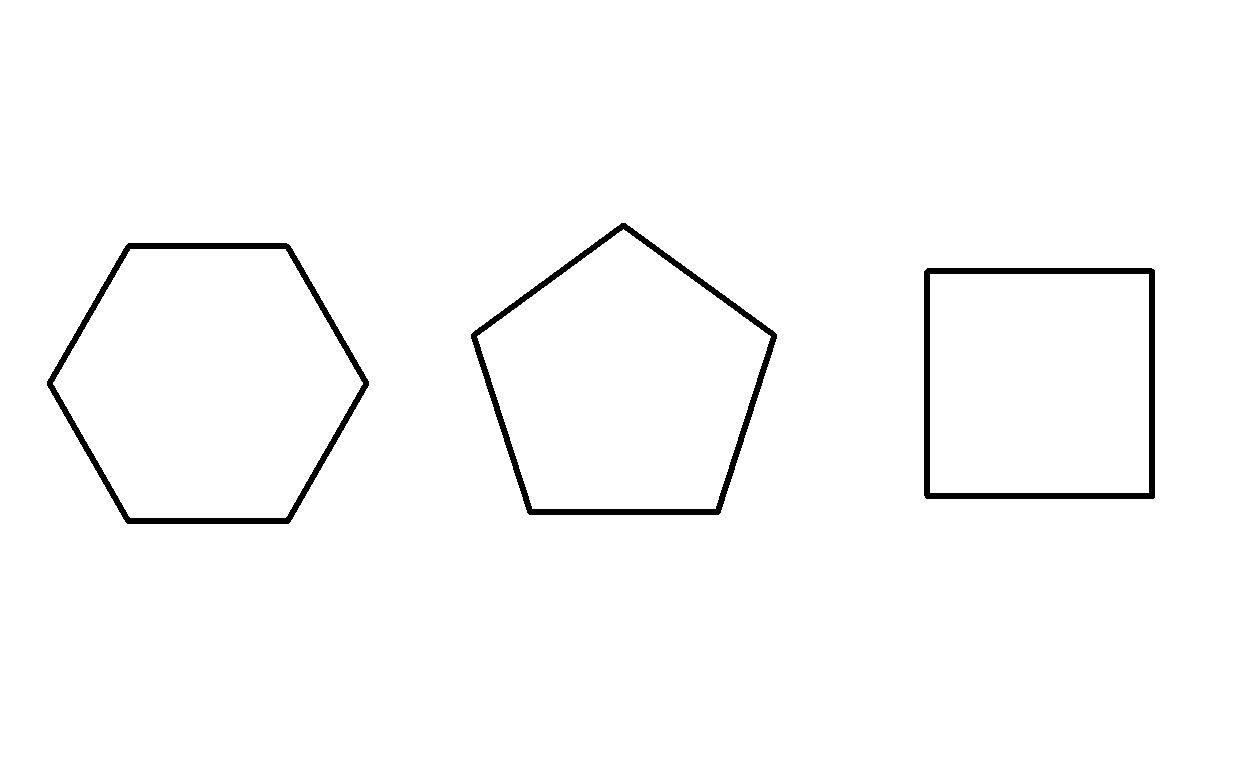
\includegraphics{matRiks-paper_files/figure-latex/permutational-1.pdf}
\caption{\label{fig:permutational}Example of shape rule transformation along a row.}
\end{figure}

By default, the order of the figures is the order with which the figures are concatenated in the starting set. If the order of the figures in the original set is changed, then the rule will adapt and the result will be consistent with the new starting order.

All the rules functions are characterized by three arguments, namely \texttt{fig},\texttt{n}, and \texttt{rules}.
The \texttt{fig} argument defines the initial figure that will be transformed.
The \texttt{n} argument defines the position of the resulting figure in the cell, in particular the number of rows or columns (depending on the directional logic) in which the outcome will be displayed.
Finally, the \texttt{rules} argument is a vector of characters that defines the type of rule.
In particular, if the vector \texttt{rules} contains the strings \texttt{inv} the default order is reversed, and it is denoted that the rule is applied reverse.
For instance, to reverse the change in size in Figure \ref(fig:incremental), the code \texttt{mat\_apply(square(size.x=10),\ hrules\ =\ "size.inv")} should be used. Figure \ref{fig:IncrementalInv} depicts the resultin sequence of squares.

\begin{figure}

{\centering 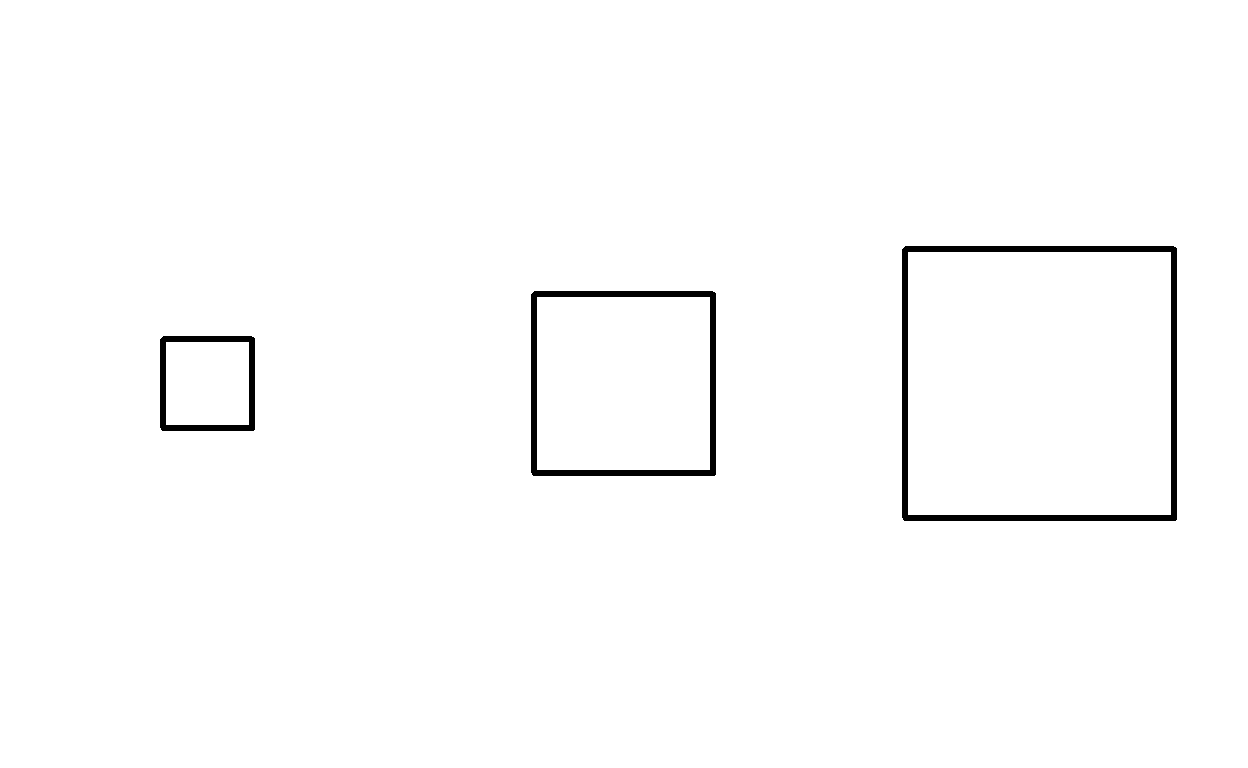
\includegraphics[width=0.7\linewidth]{matRiks-paper_files/figure-latex/IncrementalInv-1} 

}

\caption{Example of incremental rule with reverse application: Change in size}\label{fig:IncrementalInv}
\end{figure}

The reverse application of the rules can be done with permutational rules as well. By starting with the same set of figures as the one used to generate Figure \ref{fig:permutational}, the sepcification of the argument \texttt{hrules\ =\ "shape.inv"} would result in a reverse ordering of the figures across the cells (Figure \ref{fig:PermutationalInv}).

\begin{figure}

{\centering 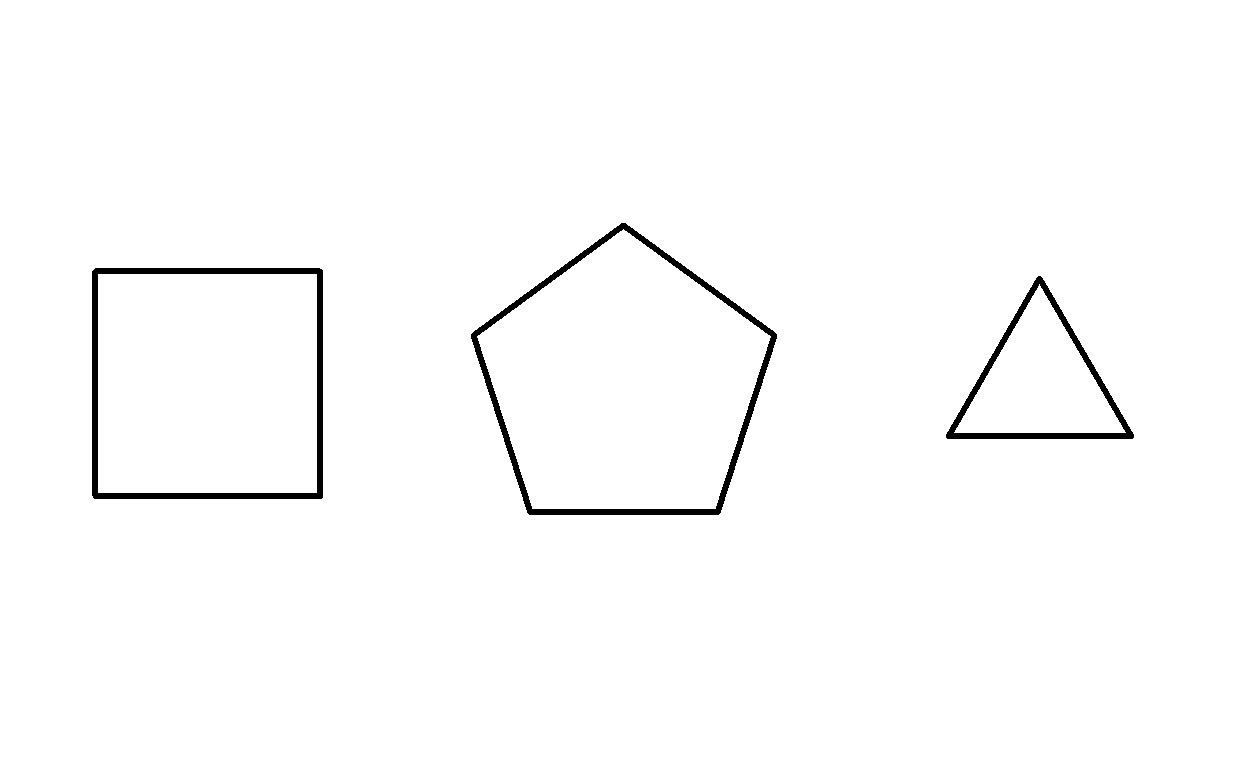
\includegraphics[width=0.7\linewidth]{matRiks-paper_files/figure-latex/PermutationalInv-1} 

}

\caption{Example of  permutational rule with reverse application: Change of shape}\label{fig:PermutationalInv}
\end{figure}

Even though rules are applied to a single figure their purpose is to be cohesive inside a matrix to allow the participant the correct options responses.

Logical rules \texttt{AND}, \texttt{OR} and \texttt{XOR} are a special case of incremental rules.
Specifically, these rules cannot be applied in reverse.

Figure @ref(fig:??) shows the flowchart of the generative procedure underlying \texttt{mat\_apply()}.
The procedure consists of three serial steps.
For the sake of simplicity, they will be illustrated for the 9-cell matrices only. A similar line of reasoning can be applied to 4-cell matrices.

The first step is to generate the named list of all the cells from \texttt{Sq1} to \texttt{Sq9}.
Each of the cells contains the initial figure defined in \texttt{Sq1}. No rule has still been applied.
For instance, considering the concatenation of figure \texttt{cof(square(),\ circle(),dot())} plotting the outcome of this step will result in the following matrix:

\begin{figure}
\centering
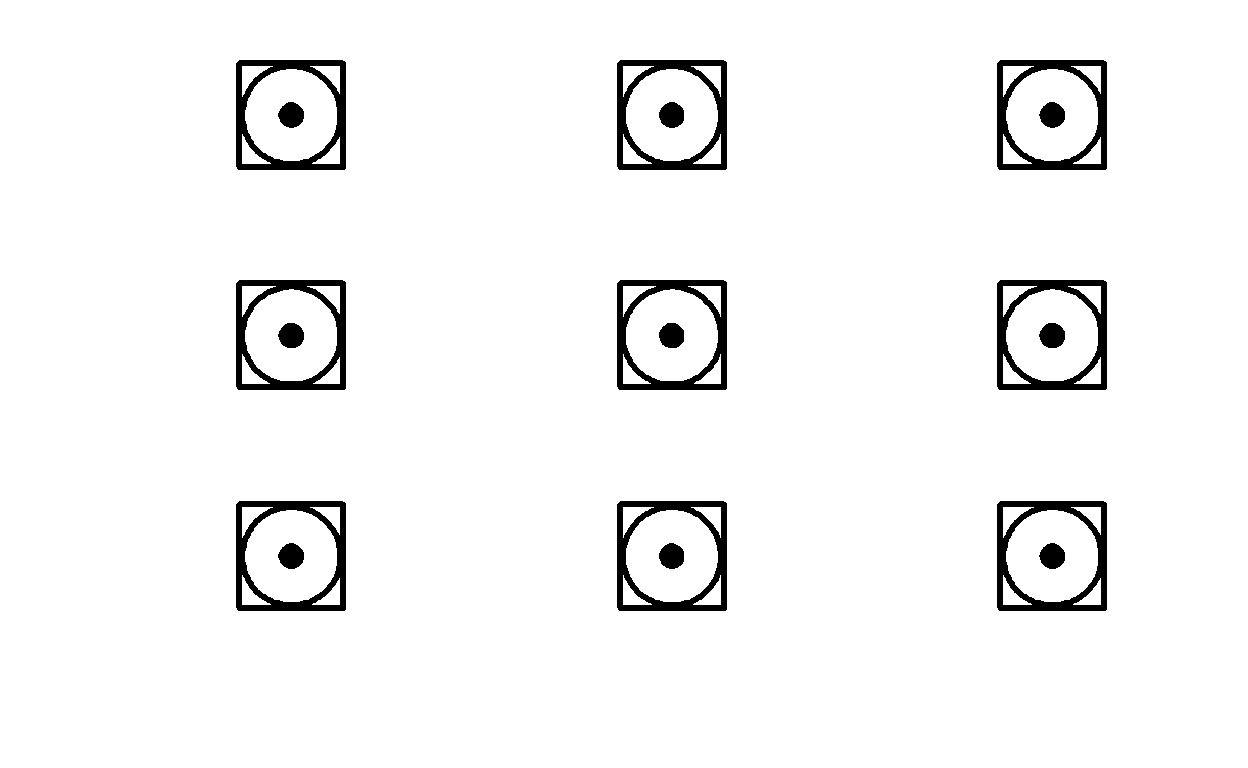
\includegraphics{matRiks-paper_files/figure-latex/examplestep1-1.pdf}
\caption{\label{fig:examplestep1}Example of outcome of the first step of the mat\_apply procedure.}
\end{figure}

Since the application of the logical rules requires a well-defined relationship between the cells of the matrix, the second step checks whether arguments \texttt{hrules} or \texttt{vrules} contain a logical rule.
If so, the procedure throws an error. An error is thrown whenever the application of a logical rule is combined with the application of a visuospatial rule, a logical rule is used for the generation of a 4-cell matrix, or if two different logical rules are applied concurrently to the same figures with different directional logic.
If only one single logical rule is applied and none of the above error-condition has been met, the procedure will generate the whole matrix in a single step.

If the test of the second step turns out to be false, the procedure enters in the third step.
In this step, the rules specified in \texttt{hrules} are applied following the horizontal directional logic (i.e., the rules are iterated among the elements horizontally.\\

The fourth step applies the rules specified in vrules following the vertical directional logic (i.e., the rules are iterated among the elements horizontally).

Since the third and forth steps are made one after another using the same rule, for instance \texttt{size}, both with a horizontal a vertical logic, the two transformation on the cells ends up to cumulate.
For instance, considering the code \texttt{mat\_apply(square(),hrules="size",\ vrules="size")}, at the end of the third step the figure in \texttt{Sq5} will be half the size of \texttt{Sq1}.
During the forth the size of \texttt{Sq5} will be halve again resulting in a figure that is a quarter of the initial \texttt{Sq1}.

It is worth mentioning that the combination of the same rule horizontally and vertically ends up in the definition of a diagonal directional logic.
In particular, if the same rule is applied in reverse in one direction and applied direct in the other, it will result in a TL-LR directional logic.
On the other hand if the same rule is direct (or reverse) in both horizontal and vertical directional logic they
will give rise to a LL-TR logic.

\hypertarget{concatenation-of-matrices}{%
\subsection{Concatenation of matrices}\label{concatenation-of-matrices}}

Matrices can be created either by applying the rule (or set of rules) with the \texttt{mat\_apply()} function (i.e., single-layer matrix) or by concatenating different matrices (i.e., multi-layer matrix). Matrices can be concatenated together with the \texttt{com()} function (i.e., \texttt{c}oncatenation \texttt{o}f \texttt{m}atrices).

Figure \ref{fig:single-matrix} and Figure \ref{fig:multi-matrix} depict a matrix created by the application of two horizontal rules (i.e., \texttt{shade} and \texttt{shape}) and one vertical rule (i.e., `rotate``). As such, the figures in the changes and their shading change horizontally, while the rotation of the figures change vertically.

\begin{figure}
\centering
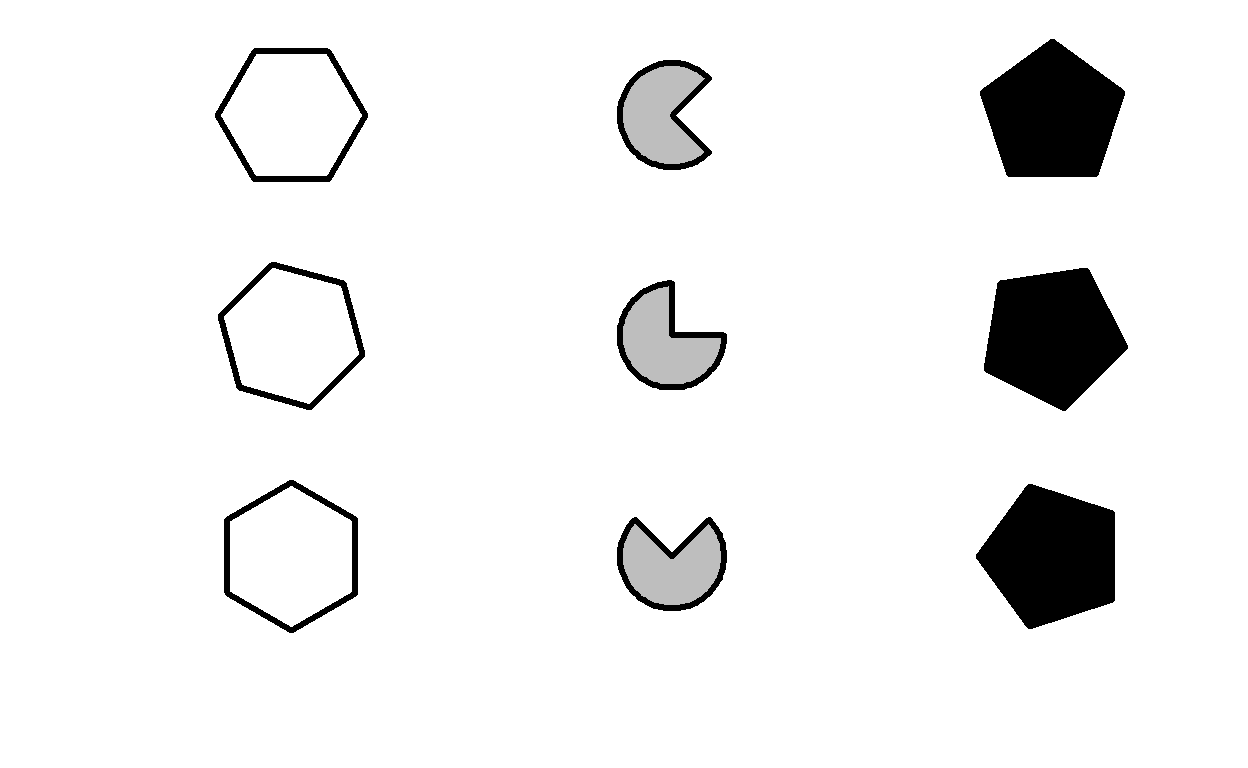
\includegraphics{matRiks-paper_files/figure-latex/single-matrix-1.pdf}
\caption{\label{fig:single-matrix}Single-layer matrix with two rules manipulated horizontally (Shape and filling) and one rules manipulated vertically (Orientation)}
\end{figure}

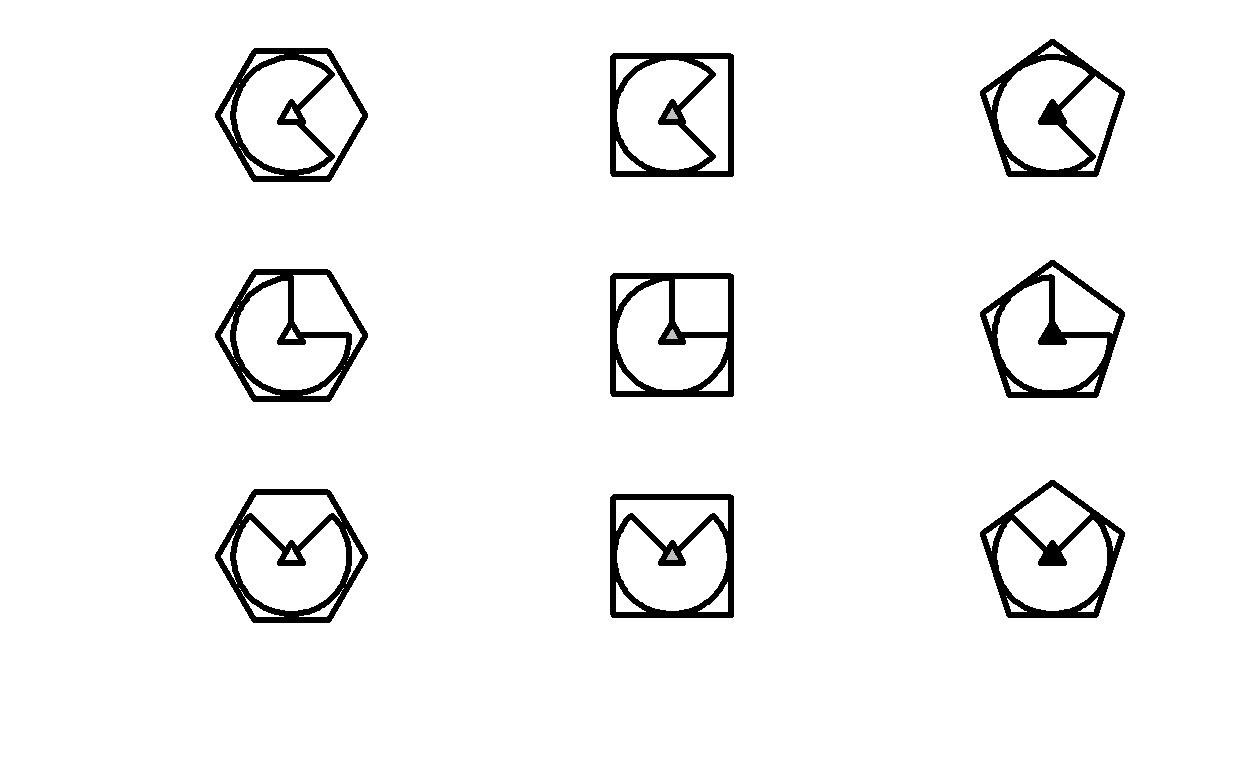
\includegraphics{matRiks-paper_files/figure-latex/multi-matrix-1.pdf}
However, in Figure \ref{fig:single-matrix} the rules are all applied to the same set of figures (i.e., \texttt{hexagon(),\ square(),\ pentagon()}) to create one single matrix, while in Figure \ref{fig:multi-matrix} the rules are separately applied to different figures to create the layers that are then combined to create the multi-layer matrix.

Each matrix concatenated to create the multi-matrix is a layer. The layering of the matrices moves from the background (considered as external) to the foreground (considered as internal). The most external layer is the background layer while the most internal layer is the foreground layer.
Layers are counted inwards \(m = 1, \ldots, M\) (where \(M\) is the total number of matrices to concatenate), such that the most external matrix (i.e., background matrix) is layer 1 and the most internal matrix (i.e., foreground matrix) is layer \(M\).\\
The following illustrates the three matrices (\(M = 3\)) that have been concatenated to create the matrix in Figure \ref{fig:multi-matrix}.

The matrix in Figure \ref{fig:multi-a} is the first layer (i.e., background layer) and it is created via the horizontal application of the changing shapes rule \texttt{shape}.

\begin{figure}
\centering
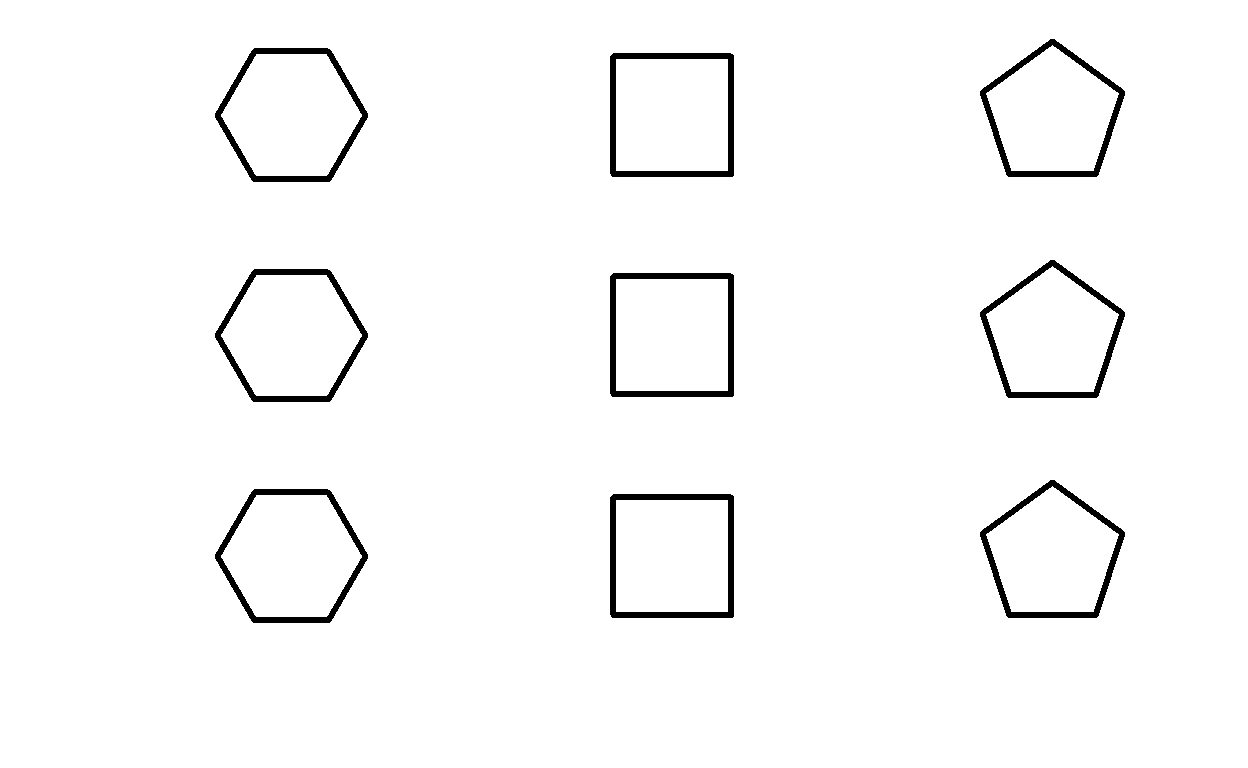
\includegraphics{matRiks-paper_files/figure-latex/multi-a-1.pdf}
\caption{\label{fig:multi-a}Layer 1 (Background matrix)}
\end{figure}

Figure \ref{fig:multi-b} is the second layer and it is created via the vertical application of the changing rotation rule \texttt{rotate}.

\begin{figure}
\centering
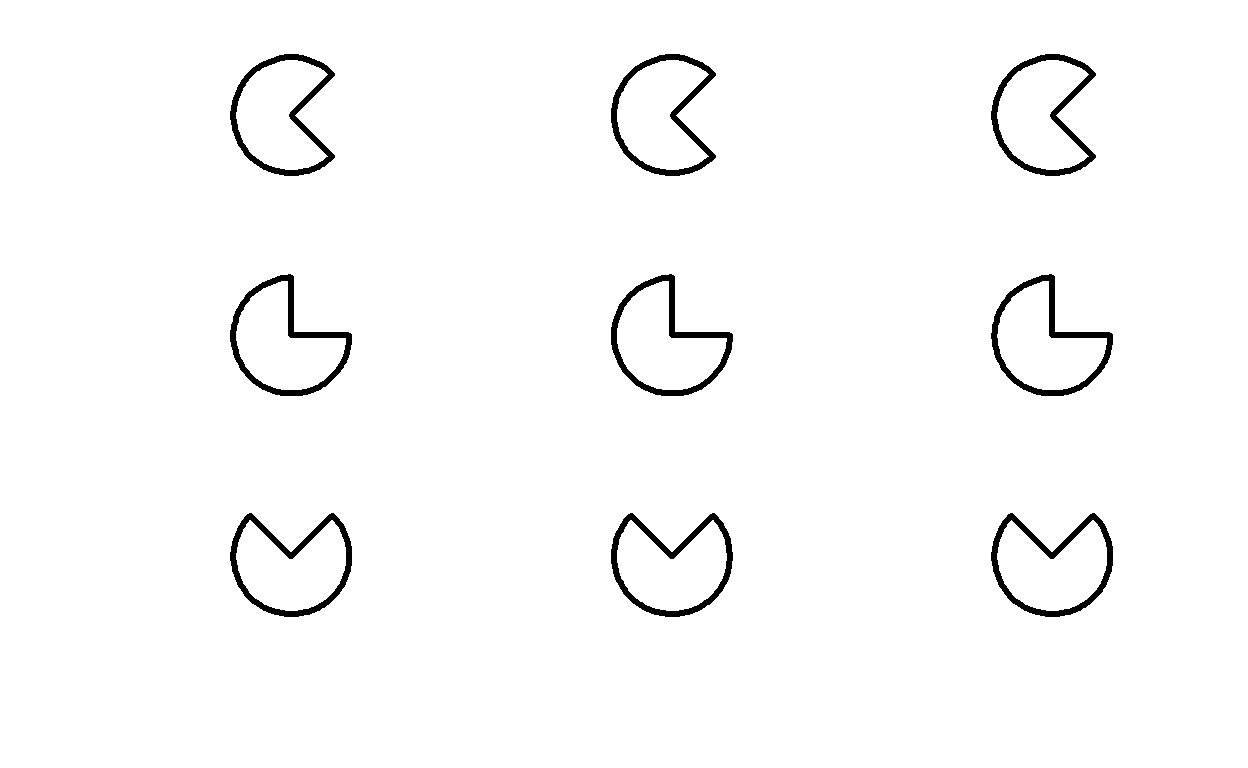
\includegraphics{matRiks-paper_files/figure-latex/multi-b-1.pdf}
\caption{\label{fig:multi-b}Layer 2}
\end{figure}

Finally, the matrix in Figure \ref{fig:multi-c} is the first layer (i.e., background layer) and it is created via the horizontal application of the changing filling rule \texttt{shade}.

\begin{figure}
\centering
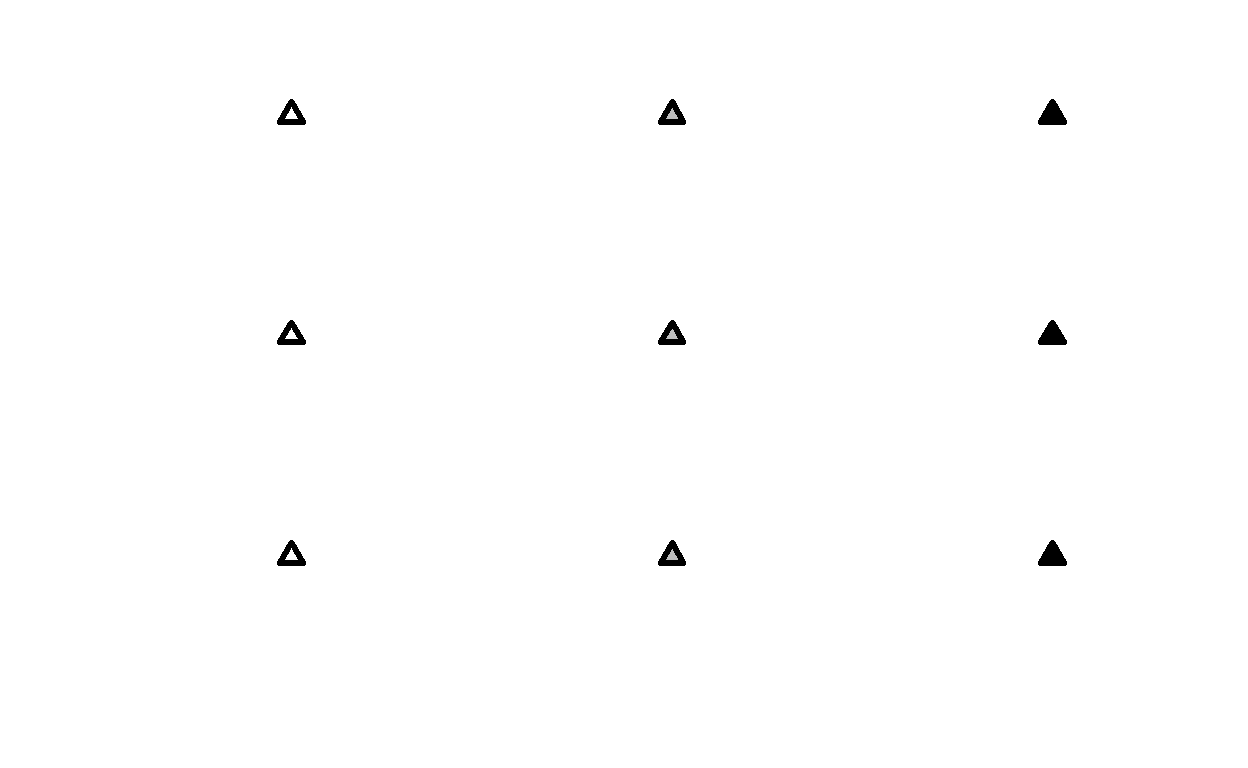
\includegraphics{matRiks-paper_files/figure-latex/multi-c-1.pdf}
\caption{\label{fig:multi-c}Layer 3 (Foreground matrix)}
\end{figure}

To create the multi-layer matrix in Figure \ref(fig:multi-matrix), the matrices in Figures \ref{fig:multi-a}, \ref{fig:multi-b}, and \ref{fig:multi-c} can be concatenated with the \texttt{com()} function, as follows:

\begin{verbatim}
com(multi_a, multi_b, multi_c)
\end{verbatim}

The matrices have to be concatenated hierarchically by following the inward order of the layers.

The hierarchy between the layers is of the uttermost importance for definition of the distractors, specifically for the generation of the incomplete correlate ones. In such cases, the manipulation of the correct response is on the most internal layer (i.e., \(M\)). Further details on the definition and on the generation of the incomplete correlate distractors of multi-layer matrices are given in section Response list.

\hypertarget{generation-of-the-response-list}{%
\subsubsection{Generation of the response list}\label{generation-of-the-response-list}}

The generation of the distractors composing the response list is constrained by the type of matrix (i.e., single-layer matrix vs.~multi-layer matrix), the rule(s) manipulated for the matrix generation, and the directional logic with which the rules are manipulated.\\
Given that, to the best of our knowledge, there is not a formal definition of the specific features of each distractor and on their applicability given the above-mentioned constrained, we started by giving a formal definition to each distractor and by considering all the possible exceptions given the constrained imposed by the matrix generated via the matrix operator.

The definitions of the distractors implemented in the \pkg{matRiks} package is reported in Table \ref{tab:dist-types-tab-static} .

\begin{table}

\caption{\label{tab:dist-types-tab-static}Definition of the distractors implemented in the \pkg{matRiks} package for $3 \times 3$ and $2 \times 2$ matrices}
\centering
\begin{tabular}[t]{l|l|l}
\hline
Distractors & \$3 \textbackslash{}times 3\$ matrices & \$2 \textbackslash{}times 2\$ matrices\\
\hline
R-Left & SQ8 & SQ3\\
\hline
R-Top & SQ6 & SQ2\\
\hline
R-diag & SQ5 & SQ1\\
\hline
Wp-Copy & SQ1 or SQ3 & SQ1\\
\hline
WP-Matrix & SQ1 or SQ3 with the superimposition of another cell. & SQ3 or SQ2 with the superimposition of the rotation of WP-Copy\\
\hline
Difference & SQ1 or SQ3, SQ4, SQ7 with the superimposition of a figure which is not manipulated in the matrix. & SQ3 or SQ1 with the superimposition of a figure that is not manipulated in the matrix\\
\hline
IC-Inc & It is the correct response with a missing element & Same as \$3\textbackslash{}times 3\$ matrices\\
\hline
 & Single-Layer: Not possible & Same as \$3\textbackslash{}times 3\$ matrices\\
\hline
 & Multi-layer: The most internal figure is removed from the correct response. & Same as \$3\textbackslash{}times 3\$ matrices\\
\hline
 & Logic matrices: The element that is removed is randomly selected. & Same as \$3\textbackslash{}times 3\$ matrices\\
\hline
IC-Neg & Color inversion of the correct response (single-layer matrix) or of one of its figures (multi-layer matrix) & Same as \$3\textbackslash{}times 3\$ matrices\\
\hline
 & Single-layer matrix:     Color inversion of the figure in the correct response & Same as \$3\textbackslash{}times 3\$ matrices\\
\hline
 & Multi-layer matrix: Color inversion of the most internal figure of the correct response & Same as \$3\textbackslash{}times 3\$ matrices\\
\hline
IC-Flip & Rotation or reflection of the correct response (single-layer matrix) or of one of its figures (multi-layer matrix) & Same as \$3\textbackslash{}times 3\$ matrices\\
\hline
 & Single-layer matrix: Reflection/Rotation of the figure in the correct response & Same as \$3\textbackslash{}times 3\$ matrices\\
\hline
 & Multi-layer matrix: Reflection/Rotation of the most internal figure of the correct response & Same as \$3\textbackslash{}times 3\$ matrices\\
\hline
IC-Scale & Resize of the correct response (single-layer matrix) or of one of its figures (multi-layer matrix) & Same as \$3\textbackslash{}times 3\$ matrices\\
\hline
 & Single-layer: Resize of the figure in the correct response & Same as \$3\textbackslash{}times 3\$ matrices\\
\hline
 & Multi-layer matrix: Only the most internal figure in the correct response is resized & Same as \$3\textbackslash{}times 3\$ matrices\\
\hline
\end{tabular}
\end{table}

The choice between cell SQ1 or cell SQ3 (WP-Copy, WP-Matrix, Difference distractors in \(3 \times 3\) matrices) depends on the number of rules and on the directional logic with which they are manipulated.
Specifically, cell SQ1 is selected when the matrix is generated via the manipulation of a single rule with V, H, or TL-LR directional logic.
If the manipulation of the single rule follows a LL-TR directional logic, then the SQ3 cell is chosen. Cell Sq3 is chosen instead of cell Sq1 when 2 rules are manipulated with all possible directional logic (i.e., VV, HH, LL-TR, and TL-LR). This is done to avoid that the WP-Copy distractors could be interpreted as IC distractors.
In other instances, the R distractors in \(3 \times 3\) matrices cannot be generated because they are equal to the correct response. For instance, if a matrix is generated with the vertical manipulation of a single rule, the R-Left distractor (SQ8) is equal to the correct response.In such instances, the distractor that is equal to the correct response is generated by the response options operator but it is covered with a thick black cross.

A similar procedures is applied for choosing which cell to use between SQ3 and SQ2 or between SQ3 and SQ1 for the generation of WP-Matrix and Difference distractors in \(2 \times 2\) matrices. In both cases, the choice depends on whether at least one rule is applied both horizontally and vertically. If the same rule is applied both horizontally and vertically, then SQ3 is chosen, otherwise SQ2 and SQ1.

The function for generating the response list (i.e., the correct response and all the distractor presented in the Table) is \texttt{response\_list()}, which results in a list of figures that correspond to each of the distractors.
For instance, the distractors of the matrix in Figure \ref{fig:single-matrix} can be obtained with:

\begin{verbatim}
response_list(single_matrix)
\end{verbatim}

The function \texttt{response\_list()} results in a named list of length 11 containing all the response options including the correct response:

\begin{verbatim}
#>  [1] "correct"    "r_diag"     "r_left"     "r_top"      "wp_copy"   
#>  [6] "wp_matrix"  "difference" "ic_neg"     "ic_flip"    "ic_size"   
#> [11] "ic_inc"
\end{verbatim}

and it can be plotted as:

\begin{verbatim}
#> Warning in ic_inc.matriks(obj): IC-Inc cannot be obtained with a single figure
\end{verbatim}

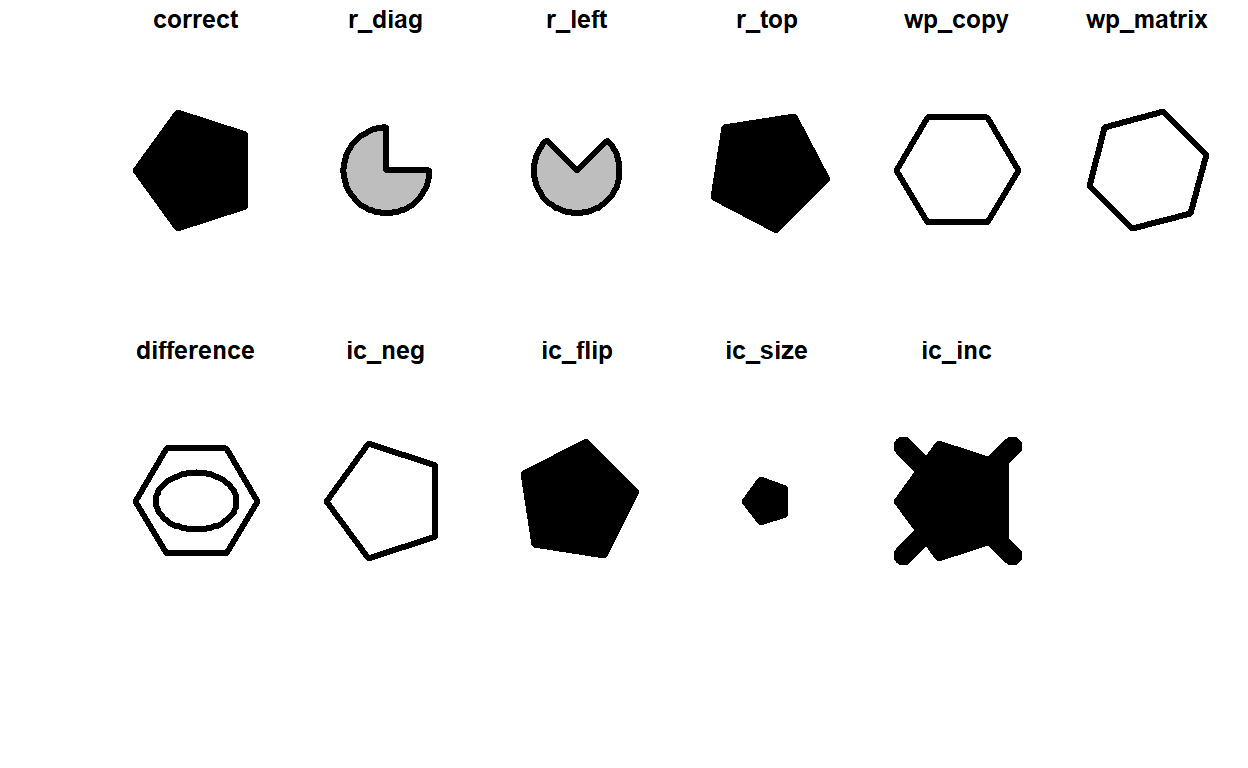
\includegraphics{matRiks-paper_files/figure-latex/unnamed-chunk-15-1.pdf}
As it can be noted, a warning has appeared and it refers to the IC-Inc distractor. As per Table \ref{tab:dist-types-tab-static} ., the distractor IC-Inc is defined as the correct response with a missing element. However, having a single-layer matrix does not allow for the removal of any element, hence the warning ``IC-Inc cannot be obtained with a single figure'' is thrown and the IC-Inc distractor is replaced by the correct response over which a black thick cross is imposed.

Given that the matrix in Figure \ref{fig:multi-matrix} is composed of three layers, it is possible to obtain also the IC-Inc distractor:

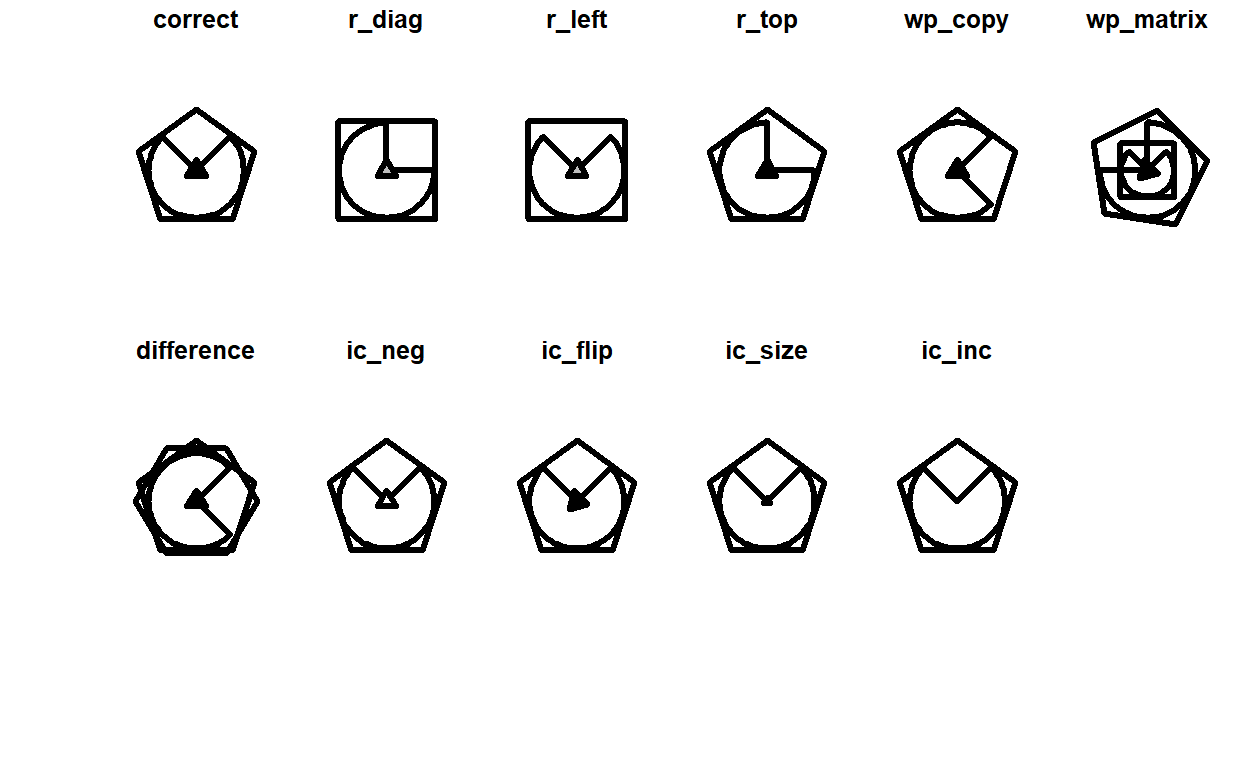
\includegraphics{matRiks-paper_files/figure-latex/unnamed-chunk-16-1.pdf}

However, the difference distractor is not well defined. The user can change the random seed for the generation of this distractor with the argument \texttt{seed()}, such that another random figure is chosen among the available ones:

\begin{verbatim}
draw(response_list(multi_matrix, seed = 7), 
     main = TRUE)
\end{verbatim}

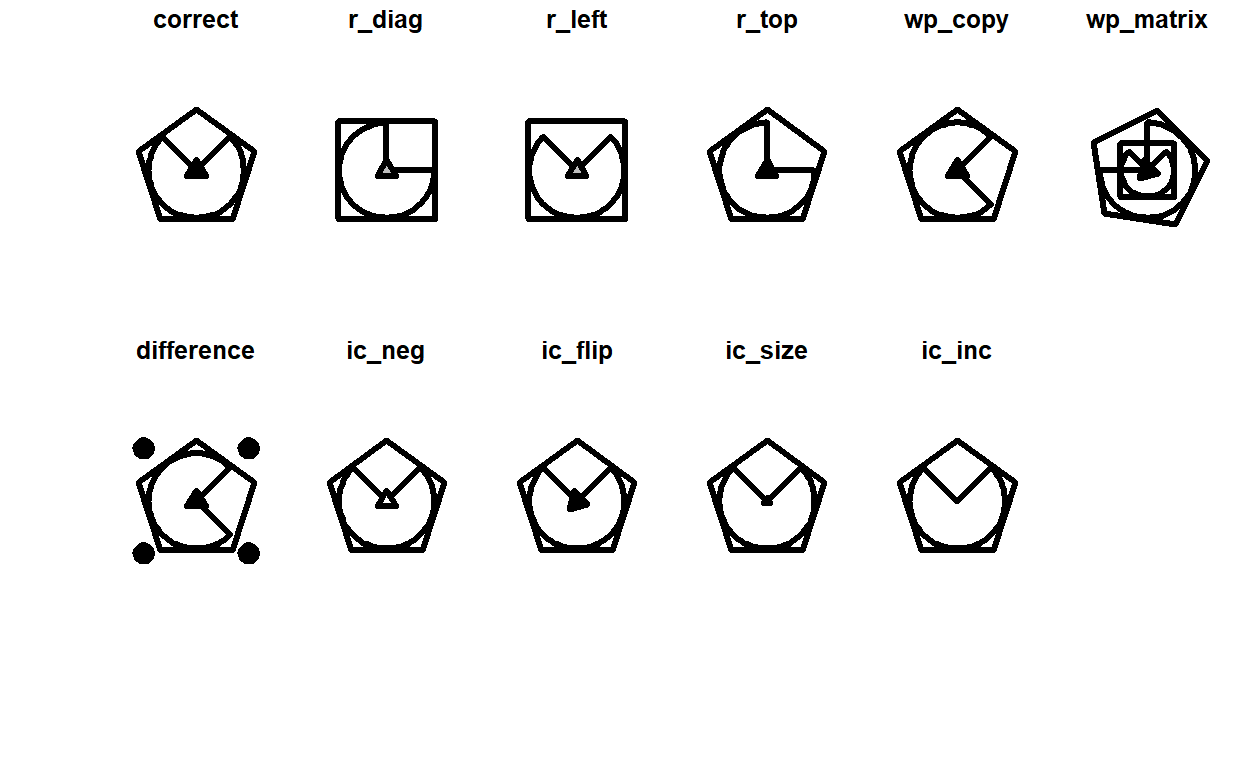
\includegraphics{matRiks-paper_files/figure-latex/unnamed-chunk-17-1.pdf}
\#\# A complete example

This section presents a complete example on how to generate a multi-layer \(3 \times 3\) matrix with logical rules and its related response options.

The first layer is generated by manipulating the AND logical rule according to an H directional logic on a square composed of 4 lines:

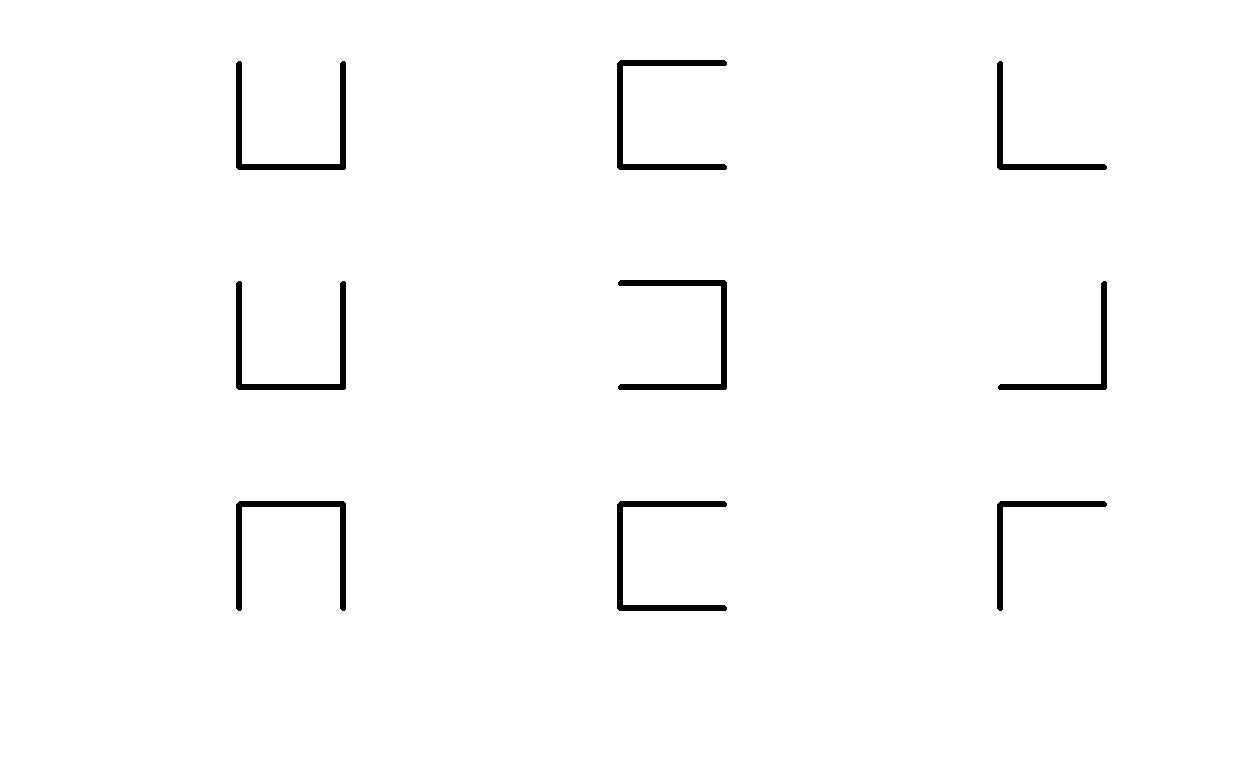
\includegraphics{matRiks-paper_files/figure-latex/unnamed-chunk-18-1.pdf}

The second layer is generated by manipulating the OR logical rule according to a V directional logic on a flower composed of 4 petals:

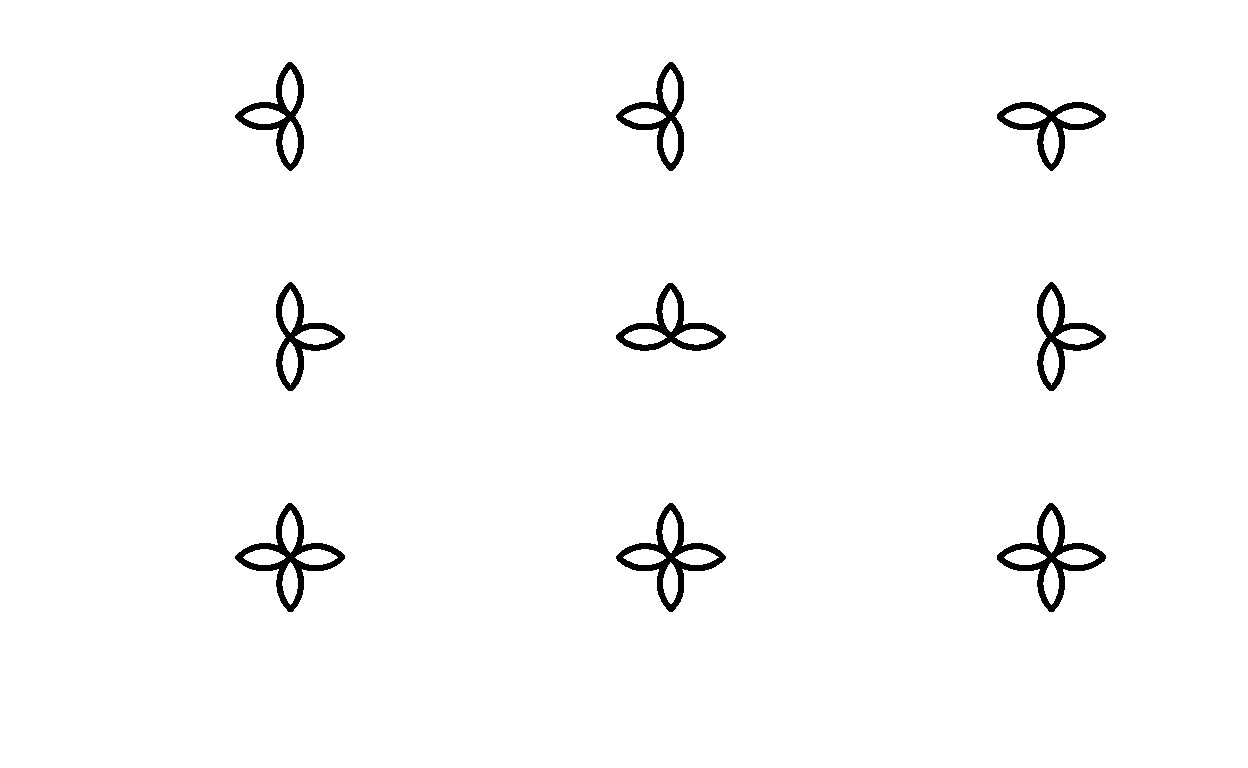
\includegraphics{matRiks-paper_files/figure-latex/unnamed-chunk-19-1.pdf}

The multi-layer matrix can be composed with the \texttt{com()} function by concatenating the two single-layer matrices:

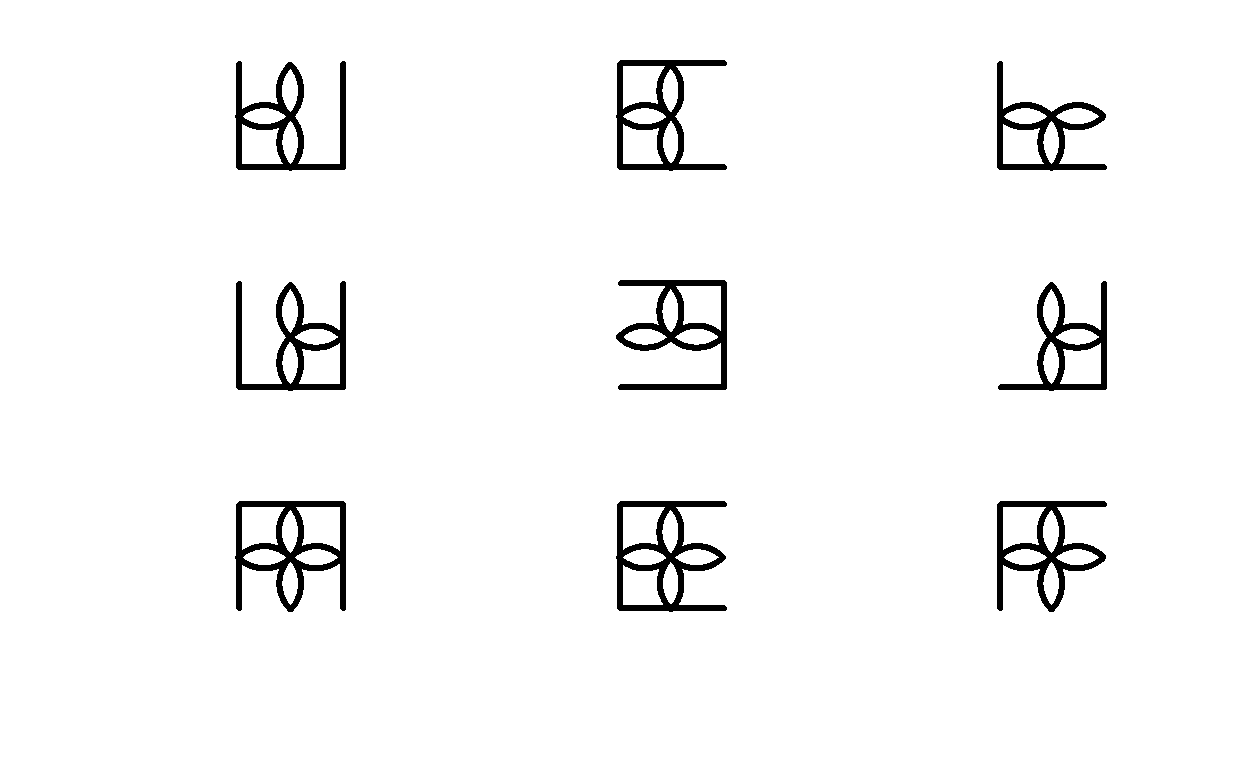
\includegraphics{matRiks-paper_files/figure-latex/unnamed-chunk-20-1.pdf}

The response options associated with the multi-layer matrix can be generated with the \texttt{response\_list()} function:

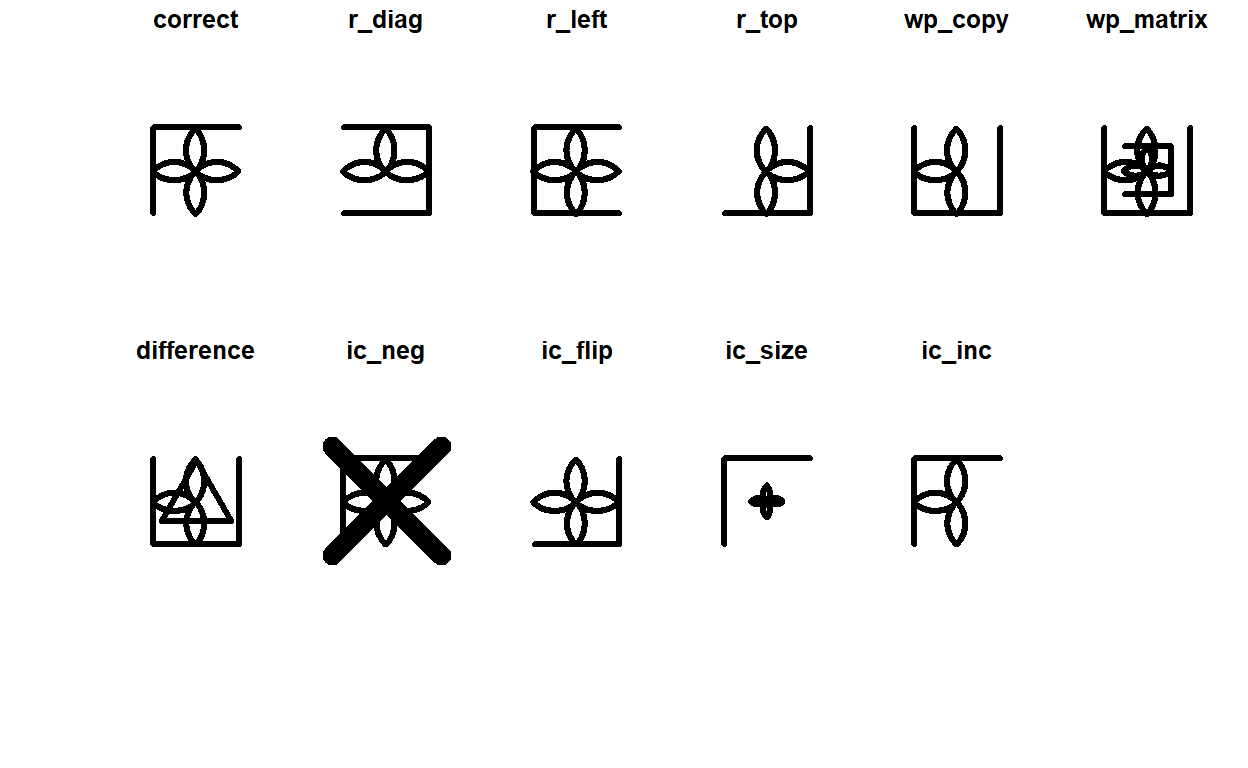
\includegraphics{matRiks-paper_files/figure-latex/unnamed-chunk-21-1.pdf}

Since the filling color the \texttt{miley} cannot be changed, the IC-Neg distractor cannot be generated and the function throws a warning and the \texttt{ic\_neg} distractor is replaced by the correct response with the superimposition of a thick black cross.
The \texttt{difference} distractor does not look good. The figure that is superimposed to the cell taken from the matrix can be changed by changing the seed in the \texttt{response\_list()} function:

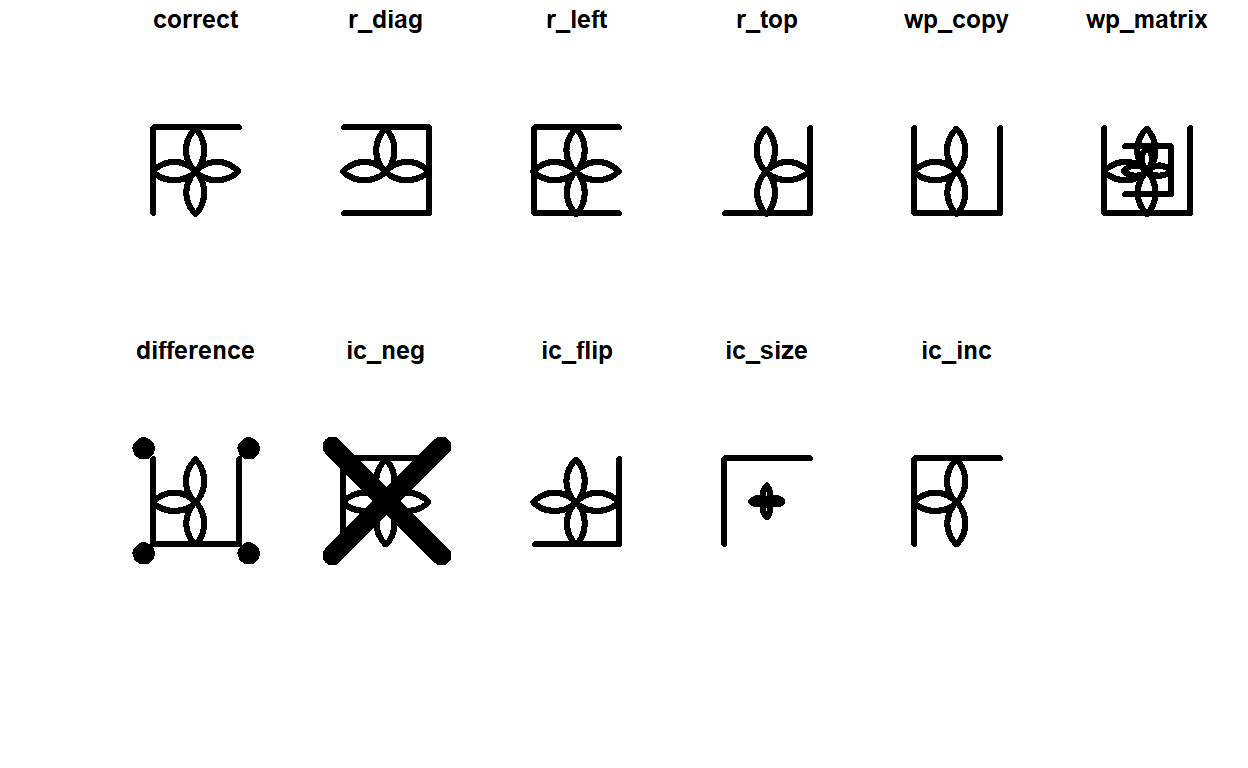
\includegraphics{matRiks-paper_files/figure-latex/unnamed-chunk-22-1.pdf}

Assuming that a response list of length 8 (the correct response along with seven distractors) is associated with the multi-layer matrix, a character vector with the labels of the chosen distractors can be specified directly in the draw function:

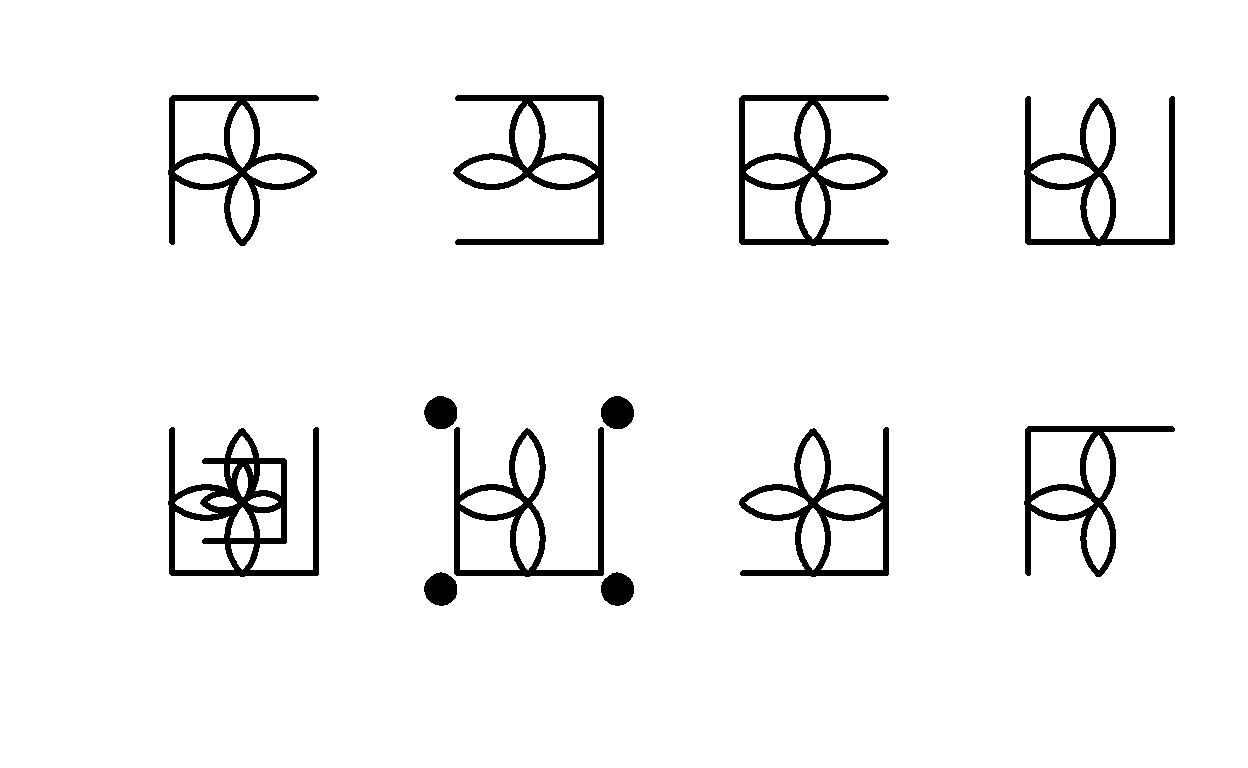
\includegraphics{matRiks-paper_files/figure-latex/unnamed-chunk-23-1.pdf}

\hypertarget{summary}{%
\section{Summary}\label{summary}}

This article briefly illustrates the functioning of the \pkg{matRiks} package for the automatic generation of Raven-like stimuli.
This package has been developed with the intention of providing the users with a flexible, open-source, and easy-to-use tool for generating Raven-like matrices according to different rules, encompassing both visuo-spatial and logical rules, along with their associated response list.

The rules for generating the matrices and for generating the distractors associated to each matrix that are implemented in the \pkg{matRiks} package derive from vast literature concerning Raven's matrices and the error patterns observed on the CPM and the APM.
As such, this package potentially provide the possibility for generating stimuli that are equivalent in terms of rules and response options to the standard Raven's stimuli. This allows for a comparison between the responses observed with the standard stimuli and those generated with the package.

This package has been developed within a broader project founded by the Italian Ministry of University and Research, which is aimed at the development of an intelligent system for the adaptive assessment of executive functions and fluid intelligence among general and clinical populations. The test used for assessment of fluid intelligence (named MatriKS) was developed following the principles of Raven's Matrices. Specifically, the stimuli composing the test have been developed with the \pkg{matRiks} package ((\textbf{mdpi?})).

This package allows for high degrees of freedom in the generation of matrices with different difficulty. For instance, it allows for the generation of stimuli that combine multiple rules by exploiting the possibility of layering multiple matrices together. Moreover, the high degree of control provided to the users allow them to thoroughly manipulate the difficulty of the matrix, for instance by adding or removing objects and combining together different rules.

The package is regularly maintained and new functions will be available in the future. As such, the users should refer to the official documentation of the package that is constantly updated.

Although the functions implemented in \pkg{matRiks} are quite straightforward and easy to use, they need a basic knowledge of the R language. To overcome this issue and allow for a wider use of the package even among people that are not familiar with R, a web application built with the \pkg{shiny} package ((\textbf{shiny?})) will be developed in the future.

\hypertarget{customizing-tooltip-design-with}{%
\section{\texorpdfstring{Customizing tooltip design with \pkg{ToOoOlTiPs}}{Customizing tooltip design with }}\label{customizing-tooltip-design-with}}

\pkg{ToOoOlTiPs} is a packages for customizing tooltips in interactive graphics, it features these possibilities.

\hypertarget{a-gallery-of-tooltips-examples}{%
\section{A gallery of tooltips examples}\label{a-gallery-of-tooltips-examples}}

The \CRANpkg{palmerpenguins} data (Horst, Hill, and Gorman 2020) features three penguin species which has a lovely illustration by Alison Horst in Figure \ref{fig:penguins-alison}.

\begin{figure}

\includegraphics[width=1\linewidth,height=0.3\textheight]{figures/penguins} \caption{Artwork by \@allison\_horst}\label{fig:penguins-alison}
\end{figure}

Table \ref{tab:penguins-tab-static} prints at the first few rows of the \texttt{penguins} data:

\begin{table}

\caption{\label{tab:penguins-tab-static}A basic table}
\centering
\fontsize{7}{9}\selectfont
\begin{tabular}[t]{l|l|r|r|r|r|l|r}
\hline
species & island & bill\_length\_mm & bill\_depth\_mm & flipper\_length\_mm & body\_mass\_g & sex & year\\
\hline
Adelie & Torgersen & 39.1 & 18.7 & 181 & 3750 & male & 2007\\
\hline
Adelie & Torgersen & 39.5 & 17.4 & 186 & 3800 & female & 2007\\
\hline
Adelie & Torgersen & 40.3 & 18.0 & 195 & 3250 & female & 2007\\
\hline
Adelie & Torgersen & NA & NA & NA & NA & NA & 2007\\
\hline
Adelie & Torgersen & 36.7 & 19.3 & 193 & 3450 & female & 2007\\
\hline
Adelie & Torgersen & 39.3 & 20.6 & 190 & 3650 & male & 2007\\
\hline
\end{tabular}
\end{table}

Figure \ref{fig:penguins-ggplot} shows an plot of the penguins data, made using the \CRANpkg{ggplot2} package.

\begin{verbatim}
penguins %>% 
  ggplot(aes(x = bill_depth_mm, y = bill_length_mm, 
             color = species)) + 
  geom_point()
\end{verbatim}

\begin{figure}
\centering
\includegraphics{matRiks-paper_files/figure-latex/penguins-ggplot-1.pdf}
\caption{\label{fig:penguins-ggplot}A basic non-interactive plot made with the ggplot2 package on palmer penguin data. Three species of penguins are plotted with bill depth on the x-axis and bill length on the y-axis. Visit the online article to access the interactive version made with the plotly package.}
\end{figure}

\hypertarget{summary-1}{%
\section{Summary}\label{summary-1}}

We have displayed various tooltips that are available in the package \pkg{ToOoOlTiPs}.

\hypertarget{references}{%
\section*{References}\label{references}}
\addcontentsline{toc}{section}{References}

\hypertarget{refs}{}
\begin{CSLReferences}{1}{0}
\leavevmode\vadjust pre{\hypertarget{ref-matRiks}{}}%
Brancaccio, Andrea, Ottavia M. Epifania, and Debora de Chiusole. 2023. \emph{matRiks: Generates Raven-Like Matrices According to Rules}. \url{https://CRAN.R-project.org/package=matRiks}.

\leavevmode\vadjust pre{\hypertarget{ref-cattell1963}{}}%
Cattell, Raymond B. 1963. {``Theory of Fluid and Crystallized Intelligence: A Critical Experiment.''} \emph{Journal of Educational Psychology} 54 (1): 1. https://doi.org/\url{https://doi.org/10.1037/h0046743}.

\leavevmode\vadjust pre{\hypertarget{ref-fort}{}}%
Forthmann, Boris, Natalie Förster, Birgit Schütze, Karin Hebbecker, Janis Flessner, Martin T. Peters, and Elmar Souvignier. 2020. {``How {Much} g {Is} in the {Distractor}? {Re}-{Thinking} {Item}-{Analysis} of {Multiple}-{Choice} {Items}.''} \emph{Journal of Intelligence} 8 (1): 11. \url{https://doi.org/10.3390/jintelligence8010011}.

\leavevmode\vadjust pre{\hypertarget{ref-palmerpenguins}{}}%
Horst, Allison Marie, Alison Presmanes Hill, and Kristen B Gorman. 2020. \emph{{palmerpenguins}: Palmer Archipelago (Antarctica) Penguin Data}. \url{https://allisonhorst.github.io/palmerpenguins/}.

\leavevmode\vadjust pre{\hypertarget{ref-kunda}{}}%
Kunda, Maithilee, Isabelle Soulières, Agata Rozga, and Ashok K. Goel. 2016. {``Error Patterns on the {Raven}'s {Standard} {Progressive} {Matrices} {Test}.''} \emph{Intelligence} 59 (November): 181--98. \url{https://doi.org/10.1016/j.intell.2016.09.004}.

\leavevmode\vadjust pre{\hypertarget{ref-raven1938}{}}%
Raven, JC ea. 1938. {``Raven's Progressive Matrices.''} \emph{Western Psychological Services} 2: 5.

\leavevmode\vadjust pre{\hypertarget{ref-raven2004}{}}%
Raven, John, and H. Raven. 2004. {``Manual for {Raven}'s {Progressive} {Matrices} and {Vocabulary} {Scales}, {Section} 3: {The} {Standard} {Progressive} {Matrices}, {Including} the {Parallel} and {Plus} {Versions}. 2000 {Edition}, Updated 2004.''} In, Section 3.

\leavevmode\vadjust pre{\hypertarget{ref-storme}{}}%
Storme, Martin, Nils Myszkowski, Simon Baron, and David Bernard. 2019. {``Same {Test}, {Better} {Scores}: {Boosting} the {Reliability} of {Short} {Online} {Intelligence} {Recruitment} {Tests} with {Nested} {Logit} {Item} {Response} {Theory} {Models}.''} \emph{Journal of Intelligence} 7 (3): 17. \url{https://doi.org/10.3390/jintelligence7030017}.

\end{CSLReferences}

\bibliography{RJreferences.bib}

\address{%
Quietest Quokka\\
University of Little Mates\\%
Department of Letter Q\\ Somewhere, Australia\\
%
\url{https://www.britannica.com/animal/quokka}\\%
\textit{ORCiD: \href{https://orcid.org/0000-1721-1511-1101}{0000-1721-1511-1101}}\\%
\href{mailto:qquo@ulm.edu}{\nolinkurl{qquo@ulm.edu}}%
}

\address{%
Bounciest Bilby\\
University of Little MatesUniversity of Aussie Animals\\%
Department of Letter Q, Somewhere, Australia\\ Department of Marsupials, Somewhere, Australia\\
%
\url{https://www.britannica.com/animal/bilby}\\%
\textit{ORCiD: \href{https://orcid.org/0000-0002-0912-0225}{0000-0002-0912-0225}}\\%
\href{mailto:bbil@ulm.edu}{\nolinkurl{bbil@ulm.edu}}%
}
